\documentclass[10pt]{article}
\usepackage[polish]{babel}
\usepackage[utf8]{inputenc}
\usepackage{polski}
\usepackage{hyperref}
\usepackage{graphicx}
\usepackage{float}
\graphicspath{{./grafiki/}}

% zmniejszenie czcionki verbatim
\makeatletter
\def\verbatim{\small\@verbatim \frenchspacing\@vobeyspaces \@xverbatim}
\makeatother

\begin{titlepage}

%Polsko-Japońska Wyższa Szkoła Technik Komputerowych
\title{Udostępnianie znakowych urządzeń fizycznych przez sieć w systemach GNU/Linux}
\author{Jakub Sokołowski}
\date{Sierpień 2013}
\maketitle

\end{titlepage}

\tableofcontents
\begin{document}

\newpage
\section{Wstęp}
\label{abstract}

Celem tego projektu jest stworzenie oprogramowania pozwalającego na współdzielenie znakowych urządzeń fizycznych za pośrednictwem sieci w dwóch zdalnych maszynach z systemem GNU/Linux. Platforma GNU/Linux udostępnia wiele możliwości współdzielenia systemów plików znajdujących się na urządzeń blokowych takich jak dyski za pomocą oprogramowania działającego z przestrzeni użytkownika i korzystającego zazwyczaj z własnego protokołu komunikacji. Najbardziej znanymi przykładami są pakiety Samba oraz NFS pozwalające na zdalny dostęp do normalnych plików.


Istnieją również metody udostępniania fizycznych urządzeń blokowych na poziomie jądra Linux przy u życiu pakietu oprogramowania NBD czyli Network Block Device. Pozwala on na stworzenie sztucznego urządzenia blokowego w zdalnym systemie które będzie się zachowywać tak jak by było to fizycznym urządzeniem podłączonym bezpośrednio do danej maszyny.

Tego typu metoda udostępniania w systemie GNU/Linux nie istnieje dla urządzeń znakowych. W celu rozwiązania tego problemu poniższy projekt implementuje moduł jądra Linux oraz program serwerowy, które w połączeniu umożliwiają współdzielenie urządzeń znakowych na stacjach połączonych przez sieć.

Projekt ten ilustruje wiele kluczowych modeli oraz standardów zdefiniowanych przez standard POSIX i wykorzystuje je w celu zaimplementowania rozwiązania które będzie przezroczyste dla jakiegokolwiek procesu który chciał by skorzystać ze zdalnego zasobu urządzenia znakowego.

\subsection{Funkcjonalność}
\label{functionality}

Sterownik jądra ma na celu stworzenie urządzenia-atrapy które będzie udawać w systemie rzeczywiste urządzenia fizyczne. Program serwerowy ma na celu odbieranie jakichkolwiek operacji wykonywanych na danym urządzeniu-atrapie i przekazanie ich do kolejnej instancji programu na zdalnej maszynie, na której znajduje się rzeczywiste urządzenie, które może odpowiedzieć na zapytania in przesłać wyniki z powrotem do urządzeniu-atrapy.

Z powodu różnorodności funkcji jakie będzie wykonywał program z przestrzeni użytkownika oraz według tradycji systemów z rodziny Unix program ten będzie od teraz nazywany demonem. Dokładny podział funkcji jakie będzie wypełniał zostanie opisany w rozdziale~\ref{Sposób implementacji programu demona}.

\subsection{Język programistyczny}
\label{language}

Z uwagi na to, iż większość kodu znajduje się w module jądra Linux głównym i jedynym językiem implementacji projektu jest język C obsługiwany przez kompilator GCC\@. Standard GCC wprowadził dużą liczbę rozszerzeń i usprawnień do podstawowego standardu ANSI C również znanego jako C89. Pisanie kodu jądra systemu wymaga dużej kontroli nad wyjątkowo specyficznymi szczegółami implementacji. Z uwagi na to Linus Torvalds podjął świadomą decyzje aby przywiązać implementacje Linuxa do jednego kompilatora - GCC - uzyskując w ten sposób liczbę dodatkowych funkcjonalności\cite{gccextensions} oraz wyższy poziom kontroli na kodem.

Kod jadra nie jest jednak napisany w czystym C. Wiele kluczowych elementów jądra, zwłaszcza te które są zależne od platformy, czyli zazwyczaj używanego procesora, jest napisanych w asemblerze. Asembler jest interpretowany przez GCC i zapisywany przy pomocy wywołania \texttt{asm}\cite{asm}.

\subsection{Biblioteki}
\label{libraries}

Wszystkie wywołania systemowe użyte w projekcie są częścią standardu POSIX\@. Implementacja komunikacji sieciowej jak i komunikacji pomiędzy przestrzenią jądra a przestrzenią użytkownika korzysta ze standardowych bibliotek C środowiska operacyjnego GNU czyli GLIBC\footnote{https://www.gnu.org/software/libc/}. Żadne dodatkowe biblioteki nie zostały wykorzystane przy rozwoju tego projektu.  Wszystkie niezbędne struktury danych takie jak tablice haszujące czy kolejki FIFO(First In, First Out) mają swoje ogólne implementacje dostępne bezpośrednio w nagłówkach jądra Linux. Do implementacji programu demona, zostały wykorzystane podstawowe funkcje interfejsu gniazd BSD dostępne w systemie Linux czyli \texttt{sendmsg}, \texttt{recvmsg} oraz \texttt{select}. Serializacja danych danych oraz implementacja protokołu komunikacji zostały zaimplementowane własnoręcznie bez użycia dodatkowych bibliotek.

\subsection{Interfejs}

Interfejs przez jaki potencjalny użytkownik będzie mógł korzystać z tego oprogramowania przyjmuje dwa podstawowe sposoby zarządzania oprogramowaniem w systemach z rodziny Unix czyli tekstowe pliki konfiguracyjne oraz argumenty przekazywane bezpośrednio do programu
demona.

\section{Organizacja pracy}

%Podział pracy na podrozdziały

\section{Teoria}
\label{theory}

Głównym tematem tej pracy jest przestrzeń jądra Linux oraz sposób w jaki obchodzi się ona z urządzeniami fizycznymi, przede wszystkim z urządzeniami znakowymi. Aby zrozumieć to zagadnienie niezbędne jest przedstawienie kilku podstawowych metod i abstrakcji, przy pomocy których jądro Linux obsługuje urządzenia. Kluczową kwestią jest zrozumienie roli plików i ich relacji do urządzeń w systemie GNU/Linux.

\subsection{Urządzenia jako pliki}
\label{devasfiles}

Tradycyjnie systemu Unix oraz jego pochodne - takie jak GNU/Linux - traktował wszystkie zasoby, które dało się odczytać lub zapisać, w jednakowy sposób, czyli jako pliki. Bez względu na to czy dany zasób jest dokumentem tekstowym, dyskiem, klawiaturą, kartą dźwiękową czy gniazdem sieciowym jest on reprezentowany w systemie jako plik. Chociaż poprawnie należało by powiedzieć, iż jest reprezentowany jako deskryptor pliku od momentu, w którym jakiś proces otworzy dany plik w celu skorzystania z jego zasobów.

Istnieje siedem podstawowych typów plików:

\begin{itemize}
\itemsep1pt\parskip0pt\parsep0pt
\item
  Pliki normalne - Najbardziej pospolity rodzaj pliku, tekstowy lub binarny, reprezentuje logicznie spójny obiekt przechowujący dane w jakimś konkretnym medium, na dysku, płycie lub w pamięci systemu.
\item
  Pliki katalogów - Katalogi również są traktowane jak pliki w systemach z rodziny Unix. Są dość specyficznymi plikami ponieważ przechowują w sobie informacje na temat innych plików jakie się w nich znajdują ale nadal są traktowane jak pliki przez system.
\item
  Pliki dowiązań symbolicznych- Specjalny rodzaj pliku, który może wskazywać na dowolny inny plik istniejący w systemie.
\item
  Pliki blokowe - Te pliki reprezentują urządzenia takie jak dyski lub czytniki optyczne. Można je znaleźć w systemie plików \texttt{/dev}.
\item
  Pliki znakowe - Najbardziej znane pliki znakowe to klawiatury lub myszki. Jest ich jednak znacznie więcej. Wirtualne terminale, modemy i jeszcze do niedawna drukarki są urządzeniami znakowymi. Również do znalezienia w systemie plików \texttt{/dev}.
\item
  Pliki potoków - Jeden z dostępnych metod komunikacji międzyprocesowej.  Istnieją nazwane i nienazwane potoki. Nazwane potoki są widoczne w systemie plików jako pliki, nienazwane nie są, nadal jednak tworzony jest dla nich deskryptor pliku w systemie.
\item
  Pliki gniazd - Gniazda BSD zazwyczaj tworzone w celu komunikacji sieciowej przy pomocy protokołów TCP lub UDP\. Pozwalają również na komunikację między procesową.
\end{itemize}

Na wszystkich tych plikach można wykonywać ten sam zestaw operacji, które zostaną dokładnie opisane w rozdziale \nameref{vfs}. W celu stworzenia modułu jądra, który tworzy specyficzny rodzaj pliku, na przykład plik blokowy, i obsługuje wykonane na nim operacji musi on implementować te operacje.

Jako że ten projekt obsługiwać będzie urządzenia znakowe reszta pracy skupi się na plikach urządzeń znakowych.

\subsection{Model VFS}
\label{vfs}

Wirtualny system plików znany przede wszystkim pod skrótem VFS(Virtual File System) to warstwa abstrakcji wprowadzona w jądrze Linux mająca na celu ujednolicenie interfejsów, przez które przestrzeń jądra oraz przestrzeń użytkownika mają dostęp do różnego rodzaju systemów plików. W dzisiejszych czasach istnieje ogromne bogactwo wszelkiego rodzaju systemów plików, od dość uniwersalnych, takich jak rodzina Ext(2,3 i 4) po stronie GNU/Linux czy FAT32 oraz NTFS po stronie produktów Microsoft, przez przystosowane do konkretnych zastosowań takich jak ZFS, BTRFS, UFS czy JFS, sieciowe systemy plików jak NFS, SMBFS i CIFS, po wirtualne systemy plików takie jak \texttt{procfs}, \texttt{devfs}, \texttt{sysfs} czy \texttt{tmpfs}. Absurdem było by implementowanie oddzielnych narzędzi do współpracy ze wszystkimi tymi systemami. W celu unifikacji sposobu implementowania dostępu oraz kontroli wszelkiego rodzaju systemów plików stworzony został model wirtualnego systemu plików VFS\. W jądrze Linux jest to prawdopodobnie system, który najbardziej czerpie z filozofii programowania obiektowego, pomimo tego iż jest ono prawie w 100\% napisane w czystym języku C które nie posiada mechanizmów obiektowości takich jak dziedziczenie czy operacje na obiektach znanych z takich języków jak C++ czy Java.

Dzięki wprowadzeniu tego modelu wszystkie sterowniki poszczególnych systemów plików muszą implementować konkretny zestaw struktur oraz funkcji, które w sposób zupełnie przezroczysty pozwalają wszystkim pozostałym elementom systemu na korzystanie z zasobów znajdujących się w tych systemach plików bez zastanawiania się na różnicami pomiędzy poszczególnymi implementacjami, formatem danych czy rodzajem nośnika na którym przechowywane są owe dane. Bez względu na to jak rzeczywiście działa dany system plików, musi on przedstawiać swoje dane przy użyciu czterech podstawowych obiektów zdefiniowanych przez model VFS:

\begin{itemize}
\item
  Blok główny(Superblock) - Jest to obiekt który zbiera w sobie wszystkie informacje o plikach i strukturze katalogów znajdujących się w danym systemie plików, jak i również jego rodzaj, przypisane do niego urządzenie oraz listę operacji które można wykonać na danym systemie plików. Blok główny bardzo często jest przechowywany w specjalnie do tego przeznaczonym sektorze dysku lub innego nośnika i posiada wszystkie informacje potrzebne by zlokalizować dane składające się na wybrany plik na przestrzeni całego nośnika. Systemy plików nie przywiązane do żadnego urządzenia fizycznego nadal muszą stworzyć obiekt bloku głównego i przechowywać go w pamięci jądra jeżeli chcą w jakimkolwiek wymiarze udostępniać swoje usługi jądru oraz procesom przestrzeni użytkownika. Blog główny definiowany jest jako struktura \texttt{super\_block}.
\item
  i-węzeł(i-node) - Każdy otwarty plik oraz katalog znajdujący się w obrębie konkretnego systemu plików reprezentowany jest przez jeden egzemplarz tego obiektu. Zbiera on w sobie wszystkie informacje potrzebne do manipulowania plikami i istnieje on tak długo jak długo plik lub katalog jest używany przez jakikolwiek proces w systemie.  Obiekt i-węzła opisuje dowolny plik, bez względu na to czy jest to zwykły plik na dysku, plik strumienia danych, urządzenie z systemu plików \texttt{/dev} czy plikowa reprezentacja atrybutów sterowników w systemie plików \texttt{/sys}. Zawiera on w sobie informacje o czasie stworzenia i modyfikacji, prawa dostępu, właścicielu, rozmiarze pliku i wiele innych informacji niezbędnych procesom do wykonywania na nich operacji. Warto od razu zwrócić uwagę, iż w systemach z rodziny Unix takich jak Linux katalogi są po prostu specyficznym rodzajem pliku, w związku z tym i-węzeł opisuje zarówno pliki jak i katalogi. Struktura która definiuje ten obiekt nazywa się \texttt{inode}.
\item
  Wpis katalogowy(Dentry) - Obiekt ten jest przeznaczony raczej do ułatwienia wyszukiwania danych w hierarchicznej strukturze katalogowej wielu systemów plików niż do opisywania rzeczywistych obiektów znajdujących się w pojedynczym systemie plików. Każdy program przestrzeni użytkownika musi korzystać ze ścieżki dostępu jeżeli chce się dostać do jakiegokolwiek zasobu w systemie plików. Przykładową ścieżką dostępu do pliku znajdującego się na płycie CD jest \texttt{/mnt/cdrom/README.txt}. W tej ścieżce dostępu znajdują się cztery wpisy katalogowe: \texttt{/}, \texttt{mnt}, \texttt{cdrom} oraz \texttt{README.txt}. Trzy pierwsze obiekty, \texttt{/} przedstawiający katalog-korzeń i \texttt{mnt} katalog znajdujący się w korzeniu oraz \texttt{cdrom} zawierający się w katalog \texttt{mnt}, znajdują się na systemie plików ext4. Jednak sam plik \texttt{README.txt} znajduje się w systemie plików płyty CDROM, ISO9660. Jądro utrzymuje bufor wpisów katalogowych, który zbiera w miarę jak procesy otwierają i używają plików dostępnych w systemie. Utrzymywanie tego typu bufora znacznie przyspiesza otwieranie wcześniej otwartych zasobów. Wpisy te reprezentowane się przez strukturę \texttt{dentry}.
\item
  Plik(File) - Tak jak i-węzeł reprezentuje każdy przynajmniej raz otwarty plik w jądrze tak obiekt pliku reprezentuje plik otwarty przez konkretny proces. Obiekt ten istnieje tak długo jak dany proces korzysta z rzeczywistego pliku i zostaje skasowany gdy proces ten użyje wywołania close() na przypisanym do niego deskryptorze pliku(file descriptor). Posiada on odwołanie do odpowiedniego obiektu i-węzła oraz zbiór informacji przydatnych przy operowaniu na pliku takich jak obecna pozycja w pliku, tryb dostępu do pliku czy zestaw praw dostępu. Nazwa jego struktury to \texttt{file} i jest to reprezentacja deskryptora pliku, który otrzymuje proces wywołując funkcje \texttt{open()} w przestrzeni jądra.
\end{itemize}

Z punktu widzenia sterowników urządzeń najbardziej kluczowymi obiektami są i-węzły oraz pliki. Obiekt pliku posiada jedną z najważniejszych struktury w całym jądrze Linux o nazwie \texttt{file\_operations}, zapisaną jako atrybut \texttt{f\_op}, która posiada kolekcję wskaźników do funkcji które pozwalają wykonywać takie operacje jak \texttt{open}, \texttt{read}, \texttt{write} czy \texttt{close}. Wszystkie urządzenia znakowe oraz blokowe muszą implementować podstawowy zestaw operacji reprezentowany przez tą strukturę i prawie każda z nich bierze jako argument obiekt pliku. Niektóre biorą również obiekt i-węzła. Dzięki temu sterownik otrzymuje niezbędne informacje odnośnie tego, który plik urządzenia został otwarty.

Struktura \texttt{file\_operations} jest kluczowym interfejsem który pozwala ukryć ogromną różnorodność urządzeń pod zestawem prostych operacji, z których każdy proces w przestrzeni użytkownika może skorzystać bez rozróżniania pomiędzy typami urządzeń. Struktura ta jest zdefiniowana razem z wcześniej wymienionymi strukturami w pliku \texttt{include/linux/fs\.h} i wygląda następująco:

\newpage
\begin{verbatim}
struct file_operations {
    struct module *owner;
    loff_t (*llseek) (struct file *, loff_t, int);
    ssize_t (*read) (struct file *, char __user *, size_t, loff_t *);
    ssize_t (*write) (struct file *, const char __user *, size_t, loff_t *);
    ssize_t (*aio_read) (struct kiocb *, const struct iovec *,
                    unsigned long, loff_t);
    ssize_t (*aio_write) (struct kiocb *, const struct iovec *,
                    unsigned long, loff_t);
    int (*readdir) (struct file *, void *, filldir_t);
    unsigned int (*poll) (struct file *, struct poll_table_struct *);
    long (*unlocked_ioctl) (struct file *, unsigned int, unsigned long);
    long (*compat_ioctl) (struct file *, unsigned int, unsigned long);
    int (*mmap) (struct file *, struct vm_area_struct *);
    int (*open) (struct inode *, struct file *);
    int (*flush) (struct file *, fl_owner_t id);
    int (*release) (struct inode *, struct file *);
    int (*fsync) (struct file *, loff_t, loff_t, int datasync);
    int (*aio_fsync) (struct kiocb *, int datasync);
    int (*fasync) (int, struct file *, int);
    int (*lock) (struct file *, int, struct file_lock *);
    ssize_t (*sendpage) (struct file *, struct page *, int, size_t,
                        loff_t *, int);
    unsigned long (*get_unmapped_area)(struct file *, unsigned long,
                        unsigned long, unsigned long, unsigned long);
    int (*check_flags)(int);
    int (*flock) (struct file *, int, struct file_lock *);
    ssize_t (*splice_write)(struct pipe_inode_info *, struct file *,
                        loff_t *, size_t, unsigned int);
    ssize_t (*splice_read)(struct file *, loff_t *,
                        struct pipe_inode_info *, size_t, unsigned int);
    int (*setlease)(struct file *, long, struct file_lock **);
    long (*fallocate)(struct file *file, int mode, loff_t offset,
              loff_t len);
    int (*show_fdinfo)(struct seq_file *m, struct file *f);
};
\end{verbatim}

W celu udostępnienia urządzenia znakowego na urządzeniu połączonym przez sieć kluczowe jest stworzenie "fałszywego" pliku urządzenia na komputerze klienckim, udostępnienie zestawu niezbędnych operacji plikowych i przekazanie wszystkich ich wywołań do maszyny posiadającej rzeczywiste urządzenie, a następnie przekazanie wyniku wywołania tej operacji z powrotem do maszyny klienckiej. Dokładniej ten proces będzie implementować ten projekt. \emph{Przekazywanie operacji plikowych z jednej maszyny do drugiej będzie główną funkcją oprogramowania stworzonego w ramach tego projektu.}

Urządzenie znakowe nie musi jednak implementować wszystkich operacji.  Przykładem operacji bezużytecznych dla plików urządzeń jest funkcja \texttt{readdir()}, która ma sens tylko i wyłącznie dla plików które są katalogami, oraz \texttt{sendpage()}, która przeznaczona jest raczej dla urządzeń sieciowych takich jak gniazda Unix. Inne operacje takie jak asynchroniczne \texttt{aio\_read()} i \texttt{aio\_write()} są rzadko implementowane dla urządzeń i prawie zawsze wartość ich wskaźnika wynosi \texttt{NULL} co sprawia, że kernel po prostu używa zwykłych funkcji \texttt{read()} oraz \texttt{write()}.

Wirtualny system plików jest kluczową abstrakcją w zrozumieniu jak jądro linux udostępnia swoje urządzenia do przestrzeni użytkownika. Prawie każde urządzenie w systemie posiada swoją reprezentacje w systemie plików \texttt{/dev} i implementuje większość lub wszystkie z tych operacji. Oczywiście istnieje szereg innych metod komunikacji z procesami specyficznych dla konkretnego rodzaju urządzeń. Na przykład karty graficzne posiadają interfejs DRI(Direct Rendering Infrastructure) która omija interfejs operacji na plikach w celu osiągnięcia jak najwyższej wydajności w obróbce grafik. Na szczęście na potrzeby zwykłych urządzeń znakowych implementacja podstawowych operacji na plikach w zupełności wystarczy.

\subsection{Model sterowników urządzeń w jądrze Linux}
\label{linuxdrivermodel}

Wszystkie urządzenia w systemie linux jak i sterowniki które implementują ich zarządzanie istnieją w jądrze w postaci dokładnie zdefiniowanych struktur, które razem tworzą model sterowników urządzań.  W modelu tym istnieją cztery podstawowe struktury, bez wykorzystania których żadne urządzenie nie ma prawa istnieć.

\begin{itemize}
\item
  Szyna(Bus) - Szyna to kanał pomiędzy procesorem a urządzeniem lub wieloma urządzeniami. Na potrzeby modelu sterowników urządzeń linux wszystkie urządzenia, bez względu na to czy fizyczne czy wirtualne, muszą przynależeć do odpowiadającej im szyny. Przykładami szyn mogą być szyny PCI, USB czy I2C. Model ten reprezentuje rzeczywiste połączenia pomiędzy szynami a urządzeniami które one kontrolują. Szyna jest reprezentowana przez strukturę \texttt{bus\_type}. Zawiera ona informacje o nazwie szyny, informacje o podłączonych urządzeniach, zbiór operacji które można na nich wykonać i wiele innych detali specyficznych dla konkretnych typów szyn.
\item
  Klasa(Class) - Jest to struktura wyższego poziomu abstrakcji która nie skupia się na niskopoziomowych kwestiach implementacji, na przykład jak dokładnie jest ono podłączone do komputera, lecz na ogólnym rodzaju urządzenia i jakie operacje da się na nim wykonać. Przykładowe klasy urządzeń to urządzenia audio, sieciowe lub dyski. Klasa reprezentowana jest w jądrze przy pomocy struktury \texttt{class}.
\item
  Sterownik(Driver) - Struktura ta opisuje i wskazuje na konkretny sterownik, również nazywany modułem, załadowany w systemie i pozwala na wykonywanie podstawowych operacji na sterownikach takich jak ich zatrzymywanie, uruchamianie, odpytywanie czy wyłączanie i usuwanie sterownika. Implementacja tego obiektu to struktura \texttt{device\_driver}, która przechowuje takie informacje jak nazwa sterownika, prywatne dane sterownika czy rodzaj szyny, z której dany sterownik obsługuje należące do niego urządzenia.
\item
  Urządzenie(Device) - Na prawie najniższym poziomie istnieje struktura urządzenia, która pozwala zdefiniować konkretną instancje obsługiwanego fizycznego lub wirtualnego urządzenia oraz plik reprezentujący je w wirtualnym systemie plików \texttt{/dev} (devfs).  Zdefiniowany jako struktura o nazwie \texttt{device} zawiera duży zbiór informacji na temat urządzenia do którego jest przypisany, w tym urządzenie macierzyste, prywatne dane modułu sterownika, szynę do której jest przyłączony, sterownik który obsługuje dane urządzenie czy numery \texttt{major}(będziemy go nazywać numerem "dur") oraz \texttt{minor}(który nazywany będzie "moll"), które identyfikują wszystkie sterowniki i urządzenia w systemie.
\end{itemize}

Wszystkie te kluczowe struktury są zdefiniowane w pliku nagłówkowym \texttt{include/linux/device.h} wraz z dużą ilością komentarzy opisujących zwierające się w nich atrybuty, struktury oraz wskaźniki do funkcji. Wraz z wieloma innymi mniej ważnymi strukturami, które są zazwyczaj atrybutami tych kluczowych struktur, tworzą one model sterowników urządzeń w jądrze Linux.

Właściwie żadnej z tych struktur programista nie tworzy lub nie wypełnia własnoręcznie. Istnieje szereg metod opakowujących, z których należy korzystać jeżeli programista chce stworzyć lub wykonać jakiekolwiek operacje na którejkolwiek z tych struktur. Ma to na celu ograniczenie błędów płynących z wywłaszczania wątków jądra jak i problemów z kompatybilności w razie przyszłych zmian w definicjach którejkolwiek z tych kluczowych struktur.

Jednym z najważniejszych elementów identyfikujących urządzenia w systemie Linux wspomniany już w opisie struktury urządzenia jest para numerów dur oraz moll, znanych w angielskim jako \texttt{major} oraz \texttt{minor}. Numery te są zapisywane kodzie źródłowym jako pojedynczy typ danych \texttt{dev\_t} który od prawie zawsze był definiowanych jako typ \texttt{unsigned long}. Pierwsze 12 bitów przeznaczone jest na numer dur a pozostałe 20 bitów na numer mol. Numer dur definiuje rodzaj sterownika a numer moll definiuje numer urządzenia obsługiwany przez dany sterownik. Wszystkie urządzenia w systemie posiadające swoją wirtualną reprezentacje w systemie plików \texttt{/dev} mają przydzielone numery dur oraz moll. Dobrym przykładem jest bardzo proste urządzenie generujące losowe dane znajdujące się pod nazwą \texttt{/dev/urandom}. Podejrzenie takiego urządzenia przy pomocy polecenia \texttt{ls -l} daje nam taki oto wynik:

\begin{verbatim}
$ ls -l /dev/urandom
crw-rw-rw- 1 root root        1,   9 Aug  7 21:34 urandom
\end{verbatim}

W miejscu, w którym w przypadku normalnych plików pojawia się wielkość widnieją dwa oddzielone przecinkiem numery. Numer 1 to dur i identyfikuje on sterownik obsługujący urządzenia urandom a numer 9 to moll i identyfikuje on konkretne urządzenie obsługiwane przez ten sterownik. Listę sterowników urządzeń znakowych oraz blokowych i przypisanych do nich numerów dur można znaleźć odczytując wirtualny plik \texttt{/proc/devices}:

\begin{verbatim}
$ cat /proc/devices
Character devices:
  1 mem
  4 /dev/vc/0
  4 tty
  ...
\end{verbatim}

Widać tutaj, że sterownik odpowiedzialny za wirtualne urządzenie \texttt{/dev/urandom} nazywa się \texttt{mem}. Jest to zrozumiałe biorąc pod uwagę, iż jest do urządzenie zupełnie wirtualne, które w razie potrzeby na żywo generuje swoje dane ze źródeł entropii w jądrze Linux.  Przy okazji warto wspomnieć, iż praktycznie wszystkie źródła entropii(losowości) w systemie Linux to urządzenia fizyczne. Na przykład używane są czasy przybycia nowych paczek do interfejsu sieciowego, a dokładnie pojawienia się przerwania IRQ związanego z danym urządzeniem w celu zwiększania entropii czyli losowości generowanych danych.  Dokładniejszy opis można znaleźć w książce Roberta Love\cite{linuxkerneldevel}.

Ogólny wgląd w model sterowników urządzeń można znaleźć w plikach dokumentacji rozprowadzanych razem z kodem źródłowym jądra w folderze \texttt{Documentation/driver-model}. Jest to jednak bardzo pobieżne spojrzenie na elementy tworzące ten system i do prawidłowego jego zrozumienia niezbędne jest czytanie samego kodu źródłowego i ciągłe konsultowanie z dokumentacją oraz bardzo często listami mailowymi związanymi z rozwijaniem jądra Linux, jako że jest to model wciąż rozwijany. Nic w jądrze Linux nie jest statyczne, i pomimo tego, że dla przeciętnego użytkownika sposób korzystania z systemu nie zmienia się zbytnio na przełomie lat pod maską trwają szeroko zakrojone prace mające na celu ulepszenie jądra Linux. Szybkość z jaką prowadzone są prace nad jądrem Linux jest jedną z jego ogromnych zalet, sprawia ona jednak, iż książki opisujące techniki programowania sterowników czy innych elementów jądra bardzo szybko stają się przestarzałe i w dużym stopniu bezużyteczne jako przewodnik dla potencjalnych przyszłych programistów jądra.

\subsection{Urządzenia znakowe}
\label{chardevs}

Urządzenia znakowe to jedne z najprostszych urządzeń jakie można znaleźć w systemie Linux. Główna różnica pomiędzy urządzeniami znakowymi a urządzeniami blokowymi wynika z użycia buforów i pamięci podręcznej oraz możliwość wykonywania operacji losowego dostępu(random access).  Urządzenia znakowe nie korzystają z buforów ani pamięci podręcznej i nie udostępniają możliwości odczytywania czy zapisywania danych w dowolnie wybranych miejscach(wyjątkiem są taśmy). Urządzenia blokowe natomiast pozwalają procesom wybrać punkt, z którego będą odczytywać i do którego będą zapisywać dane oraz korzystają z pamięci podręcznej w celu zwiększenia wydajności ,jako iż częstym zjawiskiem jest wielokrotne odczytywanie lub zapisywanie tej samej lokalizacji w medium przechowującym dane.

Podstawowym obiektem przedstawiającym urządzenia znakowe w jądrze Linux jest struktura \texttt{cdev} zdefiniowany w pliku \texttt{include/linux/cdev.h}. Wygląda ona następująco:

\begin{verbatim}
struct cdev {
    struct kobject kobj;
    struct module *owner;
    const struct file_operations *ops;
    struct list_head list;
    dev_t dev;
    unsigned int count;
};
\end{verbatim}

Jak prawie każda ważna struktura w jądrze posiada ona k-obiekt(kobject), który jest strukturą używaną przez jądro Linux do zarządzania i organizowania obiektów używanych w trakcie działania systemu. Można ten obiekt nazwać obiektem pomocniczym, ułatwia on na przykład lokalizowanie struktur na podstawie elementów, które się w nich zawierają. K-obiekty to złożony mechanizm kontroli wielu kluczowych obiektów istniejących w kodzie jądra Linux i pojawia się on w prawie każdym podsystemie jaki w nim istnieje. Dokładne wytłumaczenie tej struktury i jej działania wykracza znacznie poza zakres tego projektu i samo w sobie było by dobrym tematem na dość rozbudowaną pracę inżynierską.

Kolejnym atrybutem jest wskaźnik do struktury \texttt{module} który wskazuje na moduł sterownika obsługujący dane urządzenie znakowe.  Posiada on oczywiście strukturę \texttt{file\_operations} którą już zidentyfikowaliśmy jako niezbędny element każdego sterownika który chce udostępnić systemowi urządzenie, które obsługuje. Wskaźnik ten jest wypełniany przez sterownik podczas inicjalizacji urządzenia i jądro używa tych operacji do nadpisania domyślnych operacji na plikach które przypisane są plikowi na podstawie konfiguracji sterownika systemu plików w jakim dany plik się znajduję. Struktura \texttt{list\_head} jest pierwszym wskaźnikiem w dwukierunkowej liście obiektów i-węzłów czyli plików w systemie \texttt{/dev} połączonych z tym konkretnym urządzeniem znakowym a count to ilość elementów w liście i-węzłów.  Atrybut \texttt{dev} zapisuje przedstawione wcześniej numery dur oraz moll, które w unikalny sposób identyfikują to urządzenia oraz jego sterownik.

Struktura ta nie jest jednak tworzona i wypełniana przez programistę.  Jądro udostępnia szereg metod opakowujących, które gwarantują prawidłową obsługę błędów i kompatybilność na przestrzeni wielu wersji jądra. Oto lista najważniejszych z nich:

\begin{itemize}
\item
  \texttt{struct cdev *cdev\_alloc(void);} - Służy do alokowania przestrzeni pamięci niezbędnej dla struktury \texttt{cdev}. Zaleca się używania tej funkcji z uwagi na to, iż poza alokowaniem pamięci inicjalizuje ona również k-obiekt zawarty w \texttt{cdev}.
\item
  \texttt{void cdev\_init(struct cdev *, const struct file\_operations *);} - Odpowiada za inicjalizację struktury \texttt{cdev} przy pomocy wcześniej przygotowanej struktury reprezentującej pełen zestaw operacji plikowych implementowanych przez dany sterownik. Wszystkie sterowniki urządzeń znakowych wywołują tę funkcje z celu przygotowania do użycia struktury \texttt{cdev}, która zazwyczaj istnieje jako atrybut jakiejś wewnętrznej struktury używanej przez sterownik do przechowywania danych o implementowanym urządzeniu. Również inicjalizuje k-obiekt.
\item
  \texttt{int cdev\_add(struct cdev *, dev\_t, unsigned);} - Dodaje urządzenie reprezentowane przez strukturę \texttt{cdev} do systemu.  Funkcja ta powinno zostać wywołana wtedy i tylko wtedy gdy sterownik wykonał pomyślnie wszystkie operacje przygotowujące urządzenie do obsługi operacji, które można na nim wykonać. Po poprawnym powrocie z tej funkcji urządzenie jest uznawana za gotowe do pracy. Dodatkowo zwiększa licznik referencji zawarty w k-obiekcie.
\item
  \texttt{void cdev\_del(struct cdev *);} - Usuwa urządzenie z systemu oraz zmniejsza licznik referencji zawarty w k-obiekcie. W efekcie może to spowodować zwolnienie pamięci przeznaczonej dla struktury gdy licznik referencji osiągnie 0.
\end{itemize}

Funkcje te są zdeklarowane w pliku \texttt{include/linux/cdev.h} oraz zdefiniowane w pliku \texttt{fs/char\_dev\.c}. Poza wywołaniem funkcji \texttt{cdev\_alloc()}, \texttt{cdev\_init()} oraz \texttt{cdev\_add()} w odpowiedniej kolejności sterownik nie musi w żaden sposób operować na strukturze \texttt{cdev} aż do momentu, w którym gotowy jest usunąć urządzenie i wywołuje \texttt{cdev\_del()}. Poza tym struktura \texttt{cdev} pozostaje dostępna raczej jako repozytorium informacji o urządzeniu raczej niż aktywnie modyfikowany obiekt w trakcie działania urządzenia.

W celu przechowywania dokładniejszych danych o naszym urządzeniu sterownik będzie musiał stworzyć własną wewnętrzną strukturę reprezentującą urządzenie. Zostanie to opisane w rozdziale "\nameref{mainstructs}".

\subsection{Model oprogramowania}
\label{softmodel}

W tej chwili powinno już być jasne, że na projekt będzie musiał składać się moduł sterownika jądra Linux, który będzie odpowiedzialny za stworzenie urządzenia-atrapy i odbieranie operacji plikowych na nim wykonanych, następnie i przekazywanie ich do prawdziwego urządzenia na zdalnej maszynie, która je rzeczywiście posiada i oczekiwanie na odpowiedź. Jednak z uwagi na na wiele decyzji podjętych podczas tworzenia jądra Linux wielu programistów jądra od razu zwróciło by uwagę, iż nie należy robić w przestrzeni jądra wielu rzeczy, które wydają się jak najbardziej naturalne w przestrzeni użytkownika. Dwa takie przykłady to otwieranie i czytanie plików oraz wykonywanie połączeń sieciowych w kodzie jądra.

Istnieje wiele powodów dla których nie należy robić tych rzeczy z przestrzeni jądra. Po pierwsze czytanie plików czy odbieranie danych z gniazda wymaga konwertowania tych danych do formatu używalnego przez kod jądra. W wielu przypadkach jest to wyzwanie, które jest bardzo podatne na błędy w postaci rezerwowania zbyt dużych lub małych przestrzeni pamięci w trakcie tego procesu lub używanie wartości, które nie zostały poprawnie sprawdzone, i które mogą prowadzić do wykraczania poza przydzieloną nam pamięć. W przypadku plików problemem jest również lokalizacja pliku a w przypadku połączeń sieciowych odnalezienie poprawnego adresu, co bardzo często kończy się na statycznym ustawieniu ścieżek lub adresów w kodzie jądra. Spowoduje to potrzebę przekompilowania jądra za każdym razem gdy ta lokalizacja lub adres się zmieni.

Dodatkowym problemem jest zagrożenie bezpieczeństwa jądra. Pobieranie danych prosto ze zdalnej lokalizacji do jądra jest wręcz jawnym zaproszeniem dla wszelkiego rodzaju złośliwych użytkowników sieci do próby wykorzystania naszego modułu w celu przejęcia kontroli nad naszym systemem. Jądro powinno być ostatnim bastionem bezpieczeństwa w systemie operacyjnym i wystawianie go dla publicznego dostępu przez sieć jest bardzo złą praktyką. Popełnienie takiego błędu jest wręcz gwarancją ze kod nie zostanie przyjęty do projektu jądra Linux i najprawdopodobniej programista taki zostanie pouczony na temat podstawowych zasad projektowania systemów operacyjnych.

Z uwagi na te obiekcje projekt musi zostać podzielony na dwa odrębne elementy. Przede wszystkim moduł jądra odpowiedzialny za stronę sprzętową oraz tworzenie urządzenia atrapy i odbieranie operacji plikowych na nim wykonanych. Drugim elementem będzie program przestrzeni użytkownika odpowiedzialny za wczytanie odpowiedniej konfiguracji, połączenie się z modułem jądra oraz zdalną maszyną i ustanowieniem połączenia pomiędzy oboma końcami transakcji. Dzięki takiemu modelowi wszystkie problemy związane z wczytywaniem konfiguracji, kontrolą modułu oraz bezpieczeństwem zostaną przeniesione do warstwy użytkownika co powinno znacznie uprościć kod modułu i przyspieszyć jego działanie oraz sprawić, że końcowy produkt będzie bardziej elastyczny w użytkowaniu i konfiguracji. Poniżej przedstawiam prosty diagram opisujący przykładowe połączenie pomiędzy urządzeniem fizycznym udostępniającym swoje zasoby na maszynie udostępniającej urządzenie a urządzeniem-atrapą udającym rzeczywiste urządzenie na maszynie klienckiej:

\begin{verbatim}
                        Fizyczne urządzenie
                                |
                            Moduł jądra
                                |
                                |- Połączenie Netlink
                                |
                              Demon
                                |
                                |- Połączenie TCP/IP
                                |
                              Klient
                                |
                                |- Połączenie Netlink
                                |
                            Moduł jądra
                                |
                        Urządzenie-atrapa
\end{verbatim}

Przyjmując taki model organizacji rozszerza projekt o dodatkową warstwę komunikacji pomiędzy przestrzenią jądra a przestrzenią użytkownika co w wyraźny sposób komplikuje proces komunikacji pomiędzy urządzeniem-atrapą a rzeczywistym fizycznym urządzeniem. Jest to jednak utrudnienie niezbędne biorąc pod uwagę polisy jakie rządzą rozwojem kodu jądra Linux. Jako że chcemy udostępniać urządzenia fizyczne za pośrednictwem tego oprogramowania kluczowa jest wysoka przepustowość w przesyłaniu dużych ilości danych i niezawodność, która zapewni, że żadna operacja na pliku nie zostanie pominięta podczas przesyłania. Dokładny opis wyboru metody komunikacji znajduje się w rozdziale "\nameref{userlandcomm}".

Dodatkowo w celu zmniejszenia nakładu pracy kosztem małego zwiększenia złożoności kodu podjęta została decyzja aby zaimplementować jeden moduł jądra, który będzie odpowiedzialny za urządzenie atrapę po stronie klienta oraz rzeczywiste urządzenie po stronie serwera i jeden program przestrzeni użytkownika, który analogicznie będzie wypełniał rolę serwera oraz klienta jednocześnie. Powinno to znacznie zmniejszyć ilość linijek kodu niezbędnych do ukończenia tego projektu. Powinno to również uprości konfiguracje dla potencjalnych użytkowników z uwagi na prosty podział oprogramowania na moduł jądra oraz demona.

\section{Decyzje projektowe}

\subsection{Wybór metod komunikacji}

Model jaki został przyjęty narzuca wybór dwóch konkretnych metod komunikacji. Jednej dla komunikacji przestrzeni użytkownika z przestrzenią jądra w celu połączenia procesu serwera z załadowanym modułem jądra oraz drugiej dla komunikacji sieciowej pomiędzy dwoma instancjami procesu serwera na dwóch zdalnych maszynach. Kolejne dwa rozdziały rozważają dostępne alternatywy i wybierają metoda która najlepiej pasuje do tego projektu.

\subsubsection{Komunikacja z przestrzenią użytkownika}
\label{userlandcomm}

Ponieważ tworzenie tworzenie nowych urządzeń-atrap oraz wybieranie zdalnej maszyny do której należy się podłączyć jak i samo zadanie przesyłania operacji po sieci musi być wykonane w przestrzeni użytkownika moduł jądra musi implementować jakąś metodę komunikacji pomiędzy przestrzenią jądra a przestrzenią użytkownika. Jądro Linux udostępnia kilka możliwości prowadzenia takiej komunikacji. Mają one swoje wady i zalety, kluczowym jest więc wybranie tej, która zapewni wystarczające przenośność, przepustowość, rozszerzalność oraz szybkość w informowaniu o nowych zdarzeniach w systemie.

\begin{itemize}
\item
  Przenośność oznacza spójną strukturę danych na przestrzeni wielu różnych platform. Podstawowym problemem w komunikacji pomiędzy przestrzenią użytkownika a jądra może być na przykład wielkość słowa maszynowego które może się zmieniać w zależności od architektury na której się pracuje. Architektura x86\_64 pozwala na używane 32 bitowych słów w przestrzeni użytkownika w czasie gdy słowo w przestrzeni jądra może mieć 64 bity. Tego typu różnice są kluczowe podczas wymiany danych takich jak wskaźniki czy wartości \texttt{long}.
\item
  Przepustowość decyduje o tym jak szybko i jak duże ilości danych mogą być przekazywane pomiędzy przestrzeniami użytkownika i jądra. W przypadku pojedynczych opcji nie jest to problemem jednak istnieje wiele podsystemów jądra które wymagają transferów znacznych ilości informacji w celu ich konfiguracji. Dobrym przykładem jest system zapory ogniowej w jądrze Linux, zaawansowany routing oraz narzędzia do zarządzania kluczami w protokole IPsec.
\item
  Rozszerzalność zapewnia, że zmiany w formacie przekazywanych danych nie spowodują problemów ze wsteczną kompatybilnością ze starszymi wersjami tego samego oprogramowania. Używanie statycznych struktur lub formatów podobnych do SVC, w których poszczególne dane są po prostu rozdzielone przecinkami lub innymi znakami są trudne w modyfikowaniu bez powodowania poważnych problemów w w poprzednich wersjach. Z uwagi na to dodawanie nowych funkcjonalności może powodować wiele problemów.
\item
  Szybkość w informowaniu o zdarzeniach zazwyczaj oznacza, iż program w przestrzeni użytkownika nie jest zmuszony nieprzerwanie odpytywać jakiś element systemu w celu uzyskania informacji o zmianie stanu.  Budzony jest on sam przez jądro w celu poinformowania o zmianie stanu w urządzeniu lub module, o którym informacje próbuje uzyskać dana aplikacja przestrzeni użytkownika.
\end{itemize}

Interfejsy udostępnione przez jądro można podzielić na trzy podstawowe kategorie. Z czego pierwsza jest tak kluczowa, iż jest ona podstawą dla wszystkich pozostałych. Najbardziej pierwotnym i podstawowym sposobem komunikacji z jądrem są wywołania systemowe. System Linux implementuje ich w obecnej chwili 244 plus 16 zależnych od architektury i liczba ta nie zmienia się często z uwagi na to, iż większość wywołań systemowych było zaprojektowanych zmyślą o wypełnianiu wielu ról jednocześnie.  Większość programistów jądra stroni od dodawania nowych wywołań z uwagi na to, iż dotychczas istniejące so prawie w każdym przypadku wystarczające do każdego możliwego zastosowania oraz ponieważ raz dodane wywołanie otrzymuje swój numer identyfikacyjny który musi być umieszczonych w dwóch kluczowych plikach: \texttt{arch/sh/kernel/syscalls\_32.S} oraz \texttt{include/uapi/asm-generic/unistd.h}, i raz tam dodany nie może być usunięty. Numer ten na zawsze odpowiada temu wywołaniu i gdyby przestał być implementowany musi pozostać wśród definicji i zwracać odpowiedni kod błędu w przypadku jego użycia. Prawdą jest, że żadna inna forma komunikacji z jądrem nie jest tak szybka, co sprawia, iż jest to kuszące rozwiązanie, jednak z uwagi na wymienione zastrzeżenia tworzenie własnych wywołań systemowych i tym jak niskopoziomowa byłą by taka zmiana w jądrze jest prawie zawsze złym pomysłem i powinno być używane w absolutnej ostateczności.

Pozostałe dwie kategorie to wirtualne systemy plików takie jak \texttt{/proc} i \texttt{/sys} oraz standardowe gniazda BSD\@. Wszystkie korzystają z już omówionych wywołań systemowych i implementują istniejące modele używane do komunikacji z plikami na dyskach oraz z gniazdami sieciowymi. W przypadku systemu plików \texttt{/proc} dane pobierane są z plików w postaci czytelnej dla człowieka ale mało praktycznej dla programu, który musi przeprowadzić analizę składniową danych w celu otrzymania jakichkolwiek informacji. To samo tyczy się wysyłania danych do jądra przez pliki znajdujące się w systemie \texttt{/proc}. Dodatkowo transfer danych jest ograniczony do jednej strony pamięci oraz nie udostępnia żadnego mechanizmu do informowania programu o zdarzeniach w jądrze. Wielkość strony pamięci w jądrze jest definiowana przy pomocy makra \texttt{PAGE\_SIZE} i zazwyczaj wynosi 8192 bajtów co będzie raczej niewystarczające w przypadku przesyłania większych ilości danych. Oryginalnie system \texttt{procfs} miał być używany jedynie w celu przekazywania informacji na temat istniejących procesów, niestety w obecnej chwili jest on nadużywany do wielu innych zdań i przez cały czas trwają pracę nad przeniesieniem całej funkcjonalności do systemu plików \texttt{/sys} który udostępnia kilka usprawnienie w stosunku do jego poprzednika.

Wirtualny system plików znajdujący się w katalogu \texttt{/sys} znany również jako \texttt{sysfs} ma znacznie bardziej logiczną strukturę która pozwala na eksportowanie obiektów z przestrzeni jądra jako katalogów, ich atrybutów jako plików oraz relacji z innymi obiektami jako dowiązań symbolicznych. Posiada on również sygnalizację o wydarzeniach zaimplementowaną przy pomocy gniazd Netlink, o których będzie mowa w następnym paragrafie. Niestety system \texttt{sysfs} nadal ogranicza transfer danych do jednej strony pamięci oraz format danych potrafi zmieniać się pomiędzy wersjami jądra więc nie jest to stabilny sposób przekazywania informacji do oraz z przestrzeni użytkownika.

Metody komunikacji oparte na gniazdach BSD udostępniają znacznie bardziej przyjazny interfejs do komunikacji z przestrzenią jądra.  Bardziej prymitywną metodą z dwóch dostępnych jest używanie tak zwanych surowych gniazd typu \texttt{AF\_RAW} które pozwalają na przesyłanie struktur danych o stałym formacie oraz korzystania ze specjalnego wywołania systemowego ioctl które przyjmuje jako argument dwie wartości typu \texttt{long}, pierwszą definiującą typ komunikatu i drugą wartość samego komunikatu. Jest to nadal bardzo ograniczone jeżeli chodzi o możliwość modyfikowania i rozwijania metody komunikacji ale powala jako pierwsza metoda na przysyłanie dużych ilości danych czego nie można powiedzieć o metodach komunikacji opartych na wirtualnych systemach plików.

Ostatnią do omówienia i coraz powszechniej używaną metodą jaką udostępnia jądro linux jest protokół Netlink oparty na gniazdach BSD\@.  Jest to bezpołączeniowy protokół komunikacji opierający się na datagramach przypominający UDP, który pozwala na transfer dużych ilości danych, zapewnia taki sam poziom przenośności jak każdy inny protokół sieciowy oraz pozwala na łatwe rozwijanie metod komunikacji w miarę rozwoju projektu. Kluczowym atrybutem protokołu Netlink jest stały format zapewniający jasny podział na wiadomości, które wyróżniają się własnym numerem sekwencyjnym, typem komunikatu, zmienną długością, numerem identyfikującym proces źródłowy oraz zestawem specjalnych flag.  Flagi obecne w każdym datagramie Netlink pozwalają na dodatkową implementacje niezawodności poprzez przesyłanie wiadomości potwierdzających otrzymanie przekazu pozbywając się tym sposobem ograniczeń wynikających z niepołączeniowej natury protokołu.

Biorąc pod uwagę wszystkie możliwości protokołu Netlink jest on najlepszą opcją jeżeli chodzi o implementowanie sprawnej metody komunikacji, która pozwala na szybki transfer dowolnej ilości danych oraz łatwą identyfikacje poszczególnych wiadomości i ich typu. Aplikacje w przestrzeni użytkownika mogą korzystać z protokołu netlink tak samo jak robią to w przypadku innych protokołów sieciowych. Jedyną różnicą jest potrzeba wywołania funkcji \texttt{socket()} z rodziną gniazda ustawioną na \texttt{AF\_NETLINK} oraz typem protokołu na \texttt{SOCK\_RAW} i używaniem struktury \texttt{nlmsghdr} jako podstawy budowania każdego komunikatu przesyłanego przez gniazdo Netlink.

Oto struktura \texttt{nlmsghdr} niezbędnego nagłówka każdej wiadomości Netlink:

\begin{verbatim}
struct nlmsghdr {
    __u32 nlmsg_len;   /* długość wiadomości wliczając nagłówek */
    __u16 nlmsg_type;  /* typ wiadomości                        */
    __u16 nlmsg_flags; /* dodatkowe flagi do kontroli przepływu */
    __u32 nlmsg_seq;   /* numer sekwencyjny dla wiadomości      */
    __u32 nlmsg_pid;   /* identyfikator procesu źródłowego      */
};
\end{verbatim}

Struktura ta pozwala na łatwą organizacje własnego protokołu komunikacji przy użyciu indywidualnych wiadomości o konkretnym rodzaju, numerze identyfikacyjnym, adresie źródłowym oraz zestawie flag które pozwalają na rozdzielanie dużych wiadomości na części lub żądanie o wiadomości potwierdzające fakt odebrania przekazu po drugiej stronie pary gniazd.

Dodatkowo pokrewieństwo gniazd Netlink z gniazdami TCP/IP\@ jest kolejnym ułatwienie pozwalającym na łatwe przekazywanie komunikatów odebranych z jednego rodzaju gniazda do drugiego. Powinno to znacznie uprościć implementacje procesu demona odpowiedzialnego za przekazywanie wszystkich operacji plikowych wywołanych w module jądra do zdalnej maszyny posiadającej fizyczny egzemplarz udostępnianego urządzenia. Jest to idealne rozwiązanie na potrzeby tego projektu.

\subsubsection{Komunikacja ze zdalną maszyną}

Istnieją dwa podstawowe typy protokołów internetowych: TCP oraz UDP\. Oba spełniają kluczowe role i oba mają swoje wady. Wybranie odpowiedniego protokołu na potrzeby tego projektu będzie miało bezpośredni wpływ na niezawodność i wydajność oprogramowania.

TCP to akronim z języka angielskiego: "Transmission Control Protocol", i jest protokołem połączeniowym, co oznacza, iż obie strony połączenia utrzymują aktywne sesje tak długo jak trwa połączenia które zapewniają między innymi dostarczenie wysłanych wiadomości i ponowne ich przesyłanie w razie problemów z połączeniem oraz otrzymanie ich w poprawnej kolejności. TCP gwarantuje, że dane wysłane przez jedną stronę połączenia dotrą w całości i w poprawnej kolejności albo nie dotrą w ogóle co zazwyczaj spowoduje utratę połączenia i zakończenie sesji. Dodatkowo lub może przede wszystkim TCP pozwala na kontrole szybkości przesyłania danych poprzez modyfikowanie wielkości tak zwanego "okna". TCP na bieżąco kontroluje jak szybko druga strona jest w stanie odbierać dane, które są przesyłane i modyfikuje wielkość "okna" w celu dopasowania szybkości wysyłania danych do szybkości z jaką drugi koniec połączenie jest w stanie jest odbierać.

Nadaje się on doskonale do zastosowań, w których niedopuszczalne jest utracenie części lub całości pojedynczych pakietów z transmisji. Dzięki kontroli przepływu danych TCP daje programiście pewność, iż dane dotrą nienaruszone lub program zostanie poinformowany przez odpowiedni kod błędu o utracie połączenia. Przykładowe protokoły warstwy aplikacji, które korzystają z TCP to HTTP, SMTP, IMAP, SSH, FTP i wiele wiele innych.

Niestety protokół TCP w celu utrzymania swojego standardu niezawodności dodaje zauważalny koszt do komunikacji. Nie tylko w formie dość dużego nagłówka dodawanego do każdego pakietu TCP ale również w postaci opóźnień spowodowanych potrzebą ustanawiania sesji przez zestaw pakietów kontrolnych w tak zwanym trzy stopniowym uścisku (ang. 3-way handshake") oraz potrzeby odsyłania potwierdzeń o odebranych danych. Wszystkie te koszta sprawiają, iż TCP nie nadaje się do zastosowań, w których bardziej ceni się działanie w czasie rzeczywistym.

Między innymi z tego powodu powstał protokół UDP, z angielskiego "User Datagram Protocol". W przeciwieństwie do TCP nie gwarantuje on praktycznie niczego programiście poza tym, że będzie szybki. Nie posiada on żadnej kontroli przepływu danych, poprawności danych, sprawdzania kolejności w jakiej dane się pojawiają u odbiorcy czy metody potwierdzenia odbioru. W skrócie UDP jest protokołem bezpołączeniowym. Daje to jednak szereg zalet, które są kluczowe dla aplikacji mających do czynienia z danymi, które bardzo szybko tracą ważność. Wiele usług przesyłających obraz wideo lub komunikacje głosową korzysta z UDP z tego właśnie powodu. Aplikacje pozwalające na prowadzenie telekonferencji znacznie bardziej traciły by na używalności gdyby wszystkie dane docierały z prawie sekundowym opóźnieniem niż gdyby pare klatek na minutę zostało upuszczonych w trakcie przesyłania.

Problem z UDP polega na tym, iż sama aplikacja jest teraz odpowiedzialna za obsługiwanie otrzymanych danych w poprawnej kolejności lub weryfikowanie czy przesłane dane nie są uszkodzone. Bardzo często robienie tego jest bardziej kosztowne niż było by po prostu użycie bardziej bezpiecznego protokołu TCP\. Dodatkowo brak kontroli szybkości przepływu danych może łatwo spowodować przesycenie przepustowości sieci, z której korzysta aplikacja i doprowadzenie jej do stanu, w którym jest nieużywalna.

Pomimo tego że UDP jest powszechnie używane w wielu protokołach kluczowych dla działania sieci lokalnych oraz całego internetu takich jak DNS, DHCP, SNMP czy wiele protokołów dynamicznego routingu to wielu programistów odradza używania UDP w aplikacjach użytkowych. Istnieje tylko kilka konkretnych przykładów, w których szybkość komunikacji jest tak kluczowa, iż UDP jest naprawdę jedynym sensownym wyjściem. Głównym zastosowaniem jest komunikacja wideo oraz audio między ludźmi w czasie rzeczywistym. W większości innych przypadków UDP powoduje więcej problemów niż rozwiązuje.

Z uwagi na to podjęta została decyzja by użyć protokołu TCP w implementacji demona, który będzie przekazywał operacje na plikach urządzeń znakowych. Ponieważ absolutnie kluczowa jest kolejność w jakiej wykonywane są operacje na urządzeniach fizycznych i pominięcie jednej lub więcej operacji może mieć absolutnie katastrofalne skutki gwarancja jaką daje TCP jeżeli chodzi o dostarczenie wysłanych wiadomości jest niezbędna do poprawnego działania tego oprogramowania.

\subsection{Rozwiązanie problemu serializacji}

Każdy programista piszący programy korzystające z jakiegokolwiek protokołu komunikacji sieciowej musi dobrze zdawać sobie sprawę z problemu serializacji danych przy ich wysyłaniu oraz odbieraniu. Problem serializacji wynika z kilku kwestii. Jednym z głównych czynników jest kolejność bajtów(ang. Endianess) w liczbach całkowitych czy zmiennoprzecinkowych, których wielkość wynosi przynajmniej dwa bajty. Główne dwa rodzaje kolejności bajtów to kolejność Big-endian, w której ważniejszy bajt jest zapisywany w komórce pamięci o najniższym adresie oraz Little-endian, w którym najmniej ważny bat jest zapisywany w komórce o najniższym adresie. Kolejność ta zależy od platformy i jej architektury na jakiej dany program jest uruchamiany.

Obecnie najpopularniejsze architektury takie jak x86 czy x86-64 wykorzystują kolejność little-endian. Big-endian jest raczej formatem używanym w systemach wbudowanych lub niektórych urządzeniach przenośnych takich jak komórki. Układ Big-endian jest również znany jako "konwencja Motoroli" ponieważ ich procesory jako jedne z pierwszych używały układu Big-endian na dużą skalę. Inne przykłady to coraz rzadziej spotykane systemy IBM POWER lub IBM System 360 i 370. Dodatkowo większość popularnych architektur takich jak MIPS, SPARC, ARM, czy PowerPC pozwalają zmieniać kolejność bajtów podczas uruchamiania systemu(zmiana nie jest możliwa w trakcie działania systemu).

Dodatkowym problemem jest kwestia różnej wielkości podstawowych typów danych takich jak \texttt{int} czy \texttt{long} pomiędzy platformami. Najbardziej kluczowa jest ta różnica pomiędzy platformami 32 i 64 bitowymi które może zmienić długość takich typów jak \texttt{long} który musi być przynajmniej 32 bitowy ale może być większy.

Jądro Linux praktycznie od zawsze używa układu bajtów little-endian i większość ważnych typów danych w systemie jest definiowanych w statyczny sposób jako typy o konkretnej ilości bajtów przy pomocy makr takich jak na przykład \texttt{\_\_kernel\_uid32\_t}, które gwarantują typ danych o długości 32 bitów. Przykładem takiego typu może być powszechnie używany \texttt{size\_t} lub \texttt{loff\_t}. Dodatkowo w przestrzeni użytkownika można korzystać z typów danych takich jak \texttt{int64\_t} oraz \texttt{int32\_t} które gwarantują odpowiednią długość bitową zmiennych użytych do przesyłania danych niezależnie od platformy. Z uwagi na to, iż projekt może być używany jedynie na platformach z systemem Linux praktycznie gwarantowany jest układ little-endian oraz wielkość używanych podstawowych typów danych, podjęta została decyzja by w dużym stopniu zignorować problem konwertowania typów danych w procesie serializacji na potrzeby komunikacji pomiędzy maszynami na rzecz uproszczenia kodu i zmniejszenia nakładu pracy. Szansa użycia tego oprogramowania na systemie o innej charakterystyce jest nadal istnieje ale nie jest to bardzo prawdopodobne.

W przyszłości możliwe będzie rozszerzenie kodu o warstwę zapewniającą poprawną serializacje wszystkich danych przed przesłaniem ich z jednego modułu jądra za pośrednictwem programu serwera do drugiego modułu jądra na zdalnej maszynie.

\subsection{Sposób implementacji programu demona}
\label{daemonimplementation}

Z uwagi na to że podjęta została decyzja aby zamknąć funkcjonalność serwera oraz klienta w jednym programie przestrzeni użytkownika, który nazywać będziemy demonem, kluczowe jest rozdzielenie poszczególnych funkcji pomiędzy odrębne procesy. W przypadku normalnych programów udostępniających różnego rodzaju usługi rozsądnym pomysłem jest użycie wątków jako że zarządzanie nimi jest dość proste dzięki bibliotece wątków POSIX zwanej pthreads\footnote{\url{https://computing.llnl.gov/tutorials/pthreads/}}. Niestety specyfika naszego programu wynikająca z potrzeby komunikowania się z przestrzenią jądra za pośrednictwem gniazd Netlink sprawia że niezbędnym jest aby wątki komunikujące się z jądrem posiadały swój własny odrębny identyfikator procesu(PID). W przypadku systemów GNU/Linux wątki współdzielą identyfikator procesu z procesem macierzystym, który jest stworzył. Z tego powodu użycie wątków POSIX jest niepraktyczne.

Jednak fakt że wiadomości Netlink określają swój cel oraz źródło na podstawie identyfikatorów procesów może być znacznym ułatwieniem w implementacji programu demona. Tworząc nowy proces oraz nowe gniazdo Netlink na potrzeby komunikacji z jądrem dla każdego obsługiwanego urządzenia pozbywamy się potrzeby pisania kodu, który musiał by rozróżniać pomiędzy tym, z którego urządzenia pochodzi dany komunikat. Jeżeli użyty było by tylko jeden proces i jednego gniazda Netlink rozróżnienie takie musiało by być zaimplementowane. Ponieważ wcześniej opisany nagłówek wiadomości Netlink zawiera w sobie jedynie zmienną definiującą rodzaj komunikatu o nazwie \texttt{nlmsg\_type}, który programista może użyć w implementacji własnego protokołu komunikacji, proces demona musiał by zaglądać do samego ładunku danej wiadomości w celu zweryfikowania z jakiego urządzenia ona pochodzi. Przydzielając jeden proces do jednego urządzenia tożsamość ta jest oczywista.

Sprowadza to na właściwą ścieżkę w rozważaniach przy projektowaniu programu demona. Potrzebuje on jeden główny proces, który będzie oczekiwał na nowe połączenia od innych demonów na zdalnych maszynach nasłuchując na odpowiednim porcie TCP, jeden nowy proces na potrzeby każdego połączenia od klienta w celu obsłużenia go, czyli dla roli serwera, oraz nowy proces na potrzeby tworzenia połączeń z demonem na maszynie, która posiada rzeczywiste urządzenie, czyli dla roli klienta.

Daje to nam dwie kategorie procesów:

\begin{itemize}
\itemsep1pt\parskip0pt\parsep0pt
\item
  Proces nasłuchujący(Listener) - Przy starcie tworzy wszystkie procesy klienckie a następnie zaczyna odbierać nowe połączenia i tworzy procesy do ich obsługi.
\item
  Proces pośredniczący(Proxy) - Działa w roli klienta lub serwera i przekazuje wiadomości z jądra do zdalnej maszyny i wiadomości ze zdalnej maszyny do jądra.
\end{itemize}

\subsection{Zabezpieczenia przed paniką jądra}

\section{Implementacja}

\subsection{Podział kodu}

Z uwagi na to, że projekt jest podzielony na dwa podstawowe elementy, moduł jądra oraz demon, ważne jest aby rozdzielić ich kod w logiczny sposób aby ułatwić organizacje pracy oraz kompilacje.

Całość rozdzielona jest na trzy foldery:

\begin{itemize}
\itemsep1pt\parskip0pt\parsep0pt
\item
  \texttt{include} - Katalog ten zawiera w sobie pliki nagłówkowe, które definiują wartości niezbędne do kompilacji modułu jądra oraz programu demona. W obu przypadkach plik \texttt{Makefile} zawiera dodatkowy wpis włączający ten katalog do procesu kompilacji
\item
  \texttt{kernel} - Tutaj znajduje się cały kod modułu jądra oraz plik
  \texttt{Makefile} definiujący proces kompilacji tego modułu.
\item
  \texttt{daemon} - Posiada wszystkie pliki źródłowe składające się na program demona oraz plik \texttt{Makefile} pozwalający go zbudować.  Tutaj znajduje się również przykładowy plik \texttt{server\.conf} przedstawiający sposób konfiguracji programu.
\end{itemize}

Dodatkowo w głównym katalogu znajduje się plik \texttt{README\.md} napisany w formacie Markdown\footnote{http://daringfireball.net/projects/markdown/} dający potencjalnym użytkownikom podstawowe informacje na temat kompilacji oraz użytkowania oprogramowania.

\subsubsection{Kod modułu jądra}

Kod modułu jest podzielony na szereg plików źródłowych na podstawie ich funkcji. Oto prosty opis każdego z nich:

\begin{itemize}
\itemsep1pt\parskip0pt\parsep0pt
\item
  \texttt{dbg.h} - Definiuje makro debug() używane podczas rozwijania kodu.
\item
  \texttt{netdev.h} - Definicje wszystkich kluczowych stałych i limitów w kodzie modułu.
\item
  \texttt{main.c} - Pierwszy i ostatni kod uruchamiany w trakcie działania modułu czyli funkcje \texttt{init} oraz \texttt{exit}.
\item
  \texttt{fo.c, fo.h} - Deklaruje główną strukturę
  \texttt{file\_operations} używaną do tworzenia wszystkich urządzeń-atrap.
\item
  \texttt{netdevmgm.c, netdevmgm.h} - Kod zarządzający każdym urządzeniem atrapą oraz urządzeniem serwerem.
\item
  \texttt{netlink.c, netlink.h} - Kod odpowiedzialny za odbieranie i wysyłanie danych przez gniazdo netlink.
\item
  \texttt{fo\_access.c, fo\_access.h} - Definiuje kod zarządzający jednym procesem używającym jednego z urządzeń-atrap.
\item
  \texttt{fo\_comm.c, fo\_comm.h} - Kod, który zarządza protokołem komunikacji pomiędzy serwerem a klientem.
\item
  \texttt{fo\_recv.c, fo\_recv.h} - Funkcje wykonujące operacje plikowe na rzeczywistym urządzeniu po stronie serwera.
\item
  \texttt{fo\_send.c, fo\_send.h} - Funkcje odbierające operacje plikowe na urządzeniu-atrapie.
\end{itemize}

\subsubsection{Kod demona}

Tak samo jak moduł jądra, kod demona jest również podzielony na poszczególne pliki w celu łatwiejszej organizacji:

\begin{itemize}
\itemsep1pt\parskip0pt\parsep0pt
\item
  \texttt{netprotocol.h} - Definiuje format nagłówka każdej wiadomości przesłanej pomiędzy klientem a serwerem.
\item
  \texttt{main.c} - Kod, który analizuje argumenty z konsoli, wczytuje plik konfiguracji oraz uruchamia połączenia klienckie zdefiniowane w pliku konfiguracyjnym oraz nasłuchiwanie nowych połączeń.
\item
  \texttt{conn.c, conn.h} - Wszystko odpowiedzialne za komunikacje pomiędzy klientem a serwerem.
\item
  \texttt{netlink.c, netlink.h} - Wszystko odpowiedzialne za komunikację z modułem jądra przez gniazdo Netlink.
\item
  \texttt{proxy.c, proxy.h} - Główny kod pętli odbierający komunikaty przesyłane pomiędzy klientem a serwerem.
\item
  \texttt{signal.c, signal.h} - Kod odpowiedzialny za obsługiwanie sygnałów systemowych w bezpieczny sposób.
\end{itemize}

\subsubsection{Wspólne nagłówki}

Jedynym wspólnym plikiem nagłówkowym jest plik \texttt{include/protocol.h} definiujący szereg stałych wartości, które mają bezpośredni wpływ na sposób komunikacji modułu z programem demona oraz pomiędzy serwerem oraz klientem. Między innymi definiuje on domyślny numer portu demona przy pomocy definicji makra \texttt{NETDEV\_SERVER\_PORT} ustawionego na wartość 9999 oraz zestaw rodzajów komunikatów jakie mogą być przesyłane jako makra zaczynające się od \texttt{MSGT}.

Wprowadzając jakiekolwiek zmiany do wartości zdefiniowanym w tym pliku należy zwiększyć wartość \texttt{NETDEV\_PROTOCOL\_VERSION} o jeden aby zapobiec błędom spowodowanym przez komunikację serwera i klienta o różnych wersjach protokołu.

\subsection{Budowanie i ładowanie kodu}

\subsubsection{kbuild}

Powszechnie rozprowadzane kopie jądra Linux posiadają wbudowany system kompilowania i budowania jądra oraz ich modułów zwany \texttt{kbuild}. Jego dość obszerna dokumentacja znajduje się w folderze \texttt{Documentation/kbuild}. Z punktu widzenia projektu kluczową informacją jest sposób budowania modułów jądra. Znajduje się ona w pliku \texttt{Documentation/kbuild/modules.txt}.

System \texttt{kbuild} zbudowany jest na podstawie narzędzia GNU Make\footnote{https://www.gnu.org/software/make/} pozwala na zamknięcie wszystkich informacji niezbędnych do zbudowania modułu jądra w pliku \texttt{Makefile}. Jedyne co jest potrzebne do jego działania to już skompilowany obraz jądra oraz pliki nagłówkowe użyte podczas jego kompilacji. System ten pozwala na kompilowania modułu zarówno bezpośrednio w drzewie jądra jak i w zupełnie odrębnym folderze. Kluczowe jest jedynie posiadanie kodu oraz obrazu jądra w folderze \texttt{/usr/src/linux}.

Format plików \texttt{Makefile} używanych przez system \texttt{kbuild} jest bardzo uproszczony i nie musi zawierać normalnych wpisów definiujących cele kompilacji oraz ich zależności wraz z poleceniem, który zbuduje dany cel. Zamyka on wszystkie niezbędne informacje w dwóch podstawowych zmiennych. Oto lekko okrojony plik \texttt{Makefile} użyty do kompilacji modułu składającego się na projekt:

\begin{verbatim}
DEBUG       := -g
WARN        := -Wall -Wstrict-prototypes -Wmissing-prototypes
NOWARN      := -Wno-unused-function
INCLUDE     := -I$(src)/../include/
ccflags-y   := -O ${WARN} ${NOWARN} ${DEBUG} ${INCLUDE}

obj-m       := netdev
netdev-objs := fo_access.o fo_send.o fo_recv.o fo_comm.o fo.o
               netdevmgm.o netlink.o main.o
\end{verbatim}

Kluczowymi zmiennymi są \texttt{obj-m} oraz \texttt{netdev-objs}. Zmienna \texttt{obj-m} definiuje główny cel kompilacji czyli nasz końcowy moduł jądra. Zmienna \texttt{netdev-objs} definiuje zależności niezbędne do zbudowania pliku końcowego czyli netdev.o oraz po połączeniu plików składowych plik modułu netdev.ko. Wszystkie wymienione pliki binarne muszą posiadać takie same nazwy plików jak ich pliki źródłowe z jedyną różnicą w postaci rozszerzenia pliku. Dzięki temu system \texttt{kbuild} może łatwo znaleźć pliki źródłowe \texttt{fo\_access.c} oraz \texttt{fo\_access.h} potrzebne do zbudowania pliku \texttt{fo\_access.o} składającego się na końcowy moduł.

Zmienna \texttt{ccflags-y} pozwala programiście na przekazanie dodatkowych parametrów, które mają być użyte przez GCC, domyślny kompilator jądra, podczas budowania modułu. W skład tej zmiennej wchodzą inne zmienne w celu ułatwienia organizacji. W przypadku zmiennej WARN dodawany jest szereg opcji zwiększających czułość kompilatora na niezgodności ze standardem języka C w celu wyłapania jakichkolwiek potencjalnych problemów. Zmienna \texttt{NOWARN} pozbywa się ostrzeżeń na temat nie użytych funkcji.

Dodatkowo przy pomocy zmiennej INCLUDE i zawartej w niej opcji \texttt{-I} włączany jest katalog \texttt{include}, który znajduje się poniżej katalogów z kodem modułu oraz demona zawiera przede wszystkim plik nagłówkowy protocol.h definiujący szereg stałych wartości niezbędnych do prawidłowej komunikacji po gniazdach Netlink jak i TCP/IP\@. Bez niego nie dało by się skompilować ani modułu jądra ani demona.

Z tak zdefiniowanym plikiem \texttt{Makefile} znajdującym się w folderze z kodem modułu jądra programista musi jedynie wywołać program make. Wynikiem tej operacji będzie pełen zestaw plików binarnych z rozszerzeniem \texttt{.o} oraz plik końcowy modułu \texttt{netdev.ko}, który jest gotowy do załadowania do pamięci systemu i rozpoczęcia pracy.

Warto wspomnieć, iż program make bierze argument \texttt{-j} który pozwala na podanie ilości procesów jakie może narzędzie make stworzyć w celu szybszego skompilowania kodu źródłowego na maszynach z wieloma procesorami lub rdzeniami.

\subsubsection{insmod i rmmod}

W celu załadowania modułu do pamięci systemu i uruchomienia go w systemach GNU/Linux tradycyjnie używa się narzędzia \texttt{modprobe}. Jest to dość rozbudowany program, które potrafi zweryfikować czy moduł podany jako argument posiada jakiekolwiek zależności w postaci innych modułów jądra i załadować je w prawidłowej kolejności. Przyjmuje on również jako argument jedynie nazwę modułu.

Na potrzeby odnalezienia prawidłowego pliku modułu korzysta on z plików generowanych przez system \texttt{kbuild} umieszczanych w folderze \texttt{/lib/modules/{[}KERNEL\_VERSION{]}}. Kluczowymi plikami są \texttt{modules.alias}, \texttt{modules.dep} oraz \texttt{modules.symbols}. Przy ich użyciu zapewnia on bezbolesne zarządzanie modułami na potrzeby używanego obrazu jądra.

Niestety narzędzie to nie potrafi ładować modułów, które zostały zbudowane poza procesem kompilacji, który stworzył używany przez system obraz jądra. W tym celu programista musi użyć znacznie prostszego narzędzia o nazwie \texttt{insmod}. Jego jedyną funkcją jest załadowanie i uruchomienie modułu jądra. Jako argument przyjmuje on ścieżkę do pliku modułu z rozszerzeniem \texttt{.ko} oraz może również przyjąć zestaw opcji jeżeli dany moduł takowe definiuje.

W celu usunięcia działającego modułu z systemu programista może użyć kolejnego bardzo prostego narzędzia o nazwie \texttt{rmmod}. Przyjmuje ono jako argument nazwę modułu i kilka prostych parametrów takich jak \texttt{-f} w celu wymuszenia usunięcia modułu. Oczywiście moduł nie zostanie usunięty jeżeli nie przeprowadzi on poprawnie procesu wyjścia i nie zwolni wszystkich zarezerwowanych przez siebie zasobów.

Narzędzia insmod jak i \texttt{rmmod} dostarczają bardzo okrojone komunikaty o błędach. W celu zrozumienia problemu potrzebne jest raczej odczytanie komunikatów systemowych dostępnych przy pomocy komendy \texttt{dmesg} lub w pliku \texttt{/var/log/messages}.

\subsection{Uruchamianie i zatrzymywanie modułu}

Każdy moduł jądra musi posiadać dwie podstawowe funkcje odpowiedzialne za inicjalizację wszystkich niezbędnych zasobów i przygotowanie urządzeń fizycznych czy wirtualnych do pracy oraz zwolnienie tych wszystkich zasobów oraz urządzeń podczas zatrzymywania działania modułu. Funkcje nazywają się odpowiednio \texttt{init} oraz \texttt{exit}. Funkcje \texttt{init} można nazwać ekwiwalentem głównej funkcji \texttt{main()}, od której każdy program C zaczyna swoje działanie.

W module \texttt{netdev} zdefiniowane one są w pliku \texttt{kernel/main.c} i nazywają się \texttt{netdev\_init()} oraz \texttt{netdev\_exit()}. Rejestruje się te specjalne funkcje przy pomocy dwóch makr przeznaczonych do tego właśnie zadania:

\begin{verbatim}
module_exit(netdev_exit);
module_init(netdev_init);
\end{verbatim}

Bez wyznaczenia funkcji inicjującej moduł oraz funkcji zamykającej go jądro nie wiedziało by jak taki moduł uruchomić. Jest to absolutne minimum jaki musi wykonać każda implementacja jakiegokolwiek modułu jądra Linux.

\newpage
Funkcja inicjująca moduł \texttt{netdev} wykonuje kilka podstawowych czynności niezbędny do rozpoczęcia pracy. Rezerwuje numery dur oraz moll, klasę urządzeń jakie będzie obsługiwał i inicjuje wszystkie struktury niezbędne do normalnego działania modułu. Oto kod funkcji \texttt{netdev\_init()}:

\begin{verbatim}
static int __init netdev_init(void) { /* constructor */
    int err;
    int first_minor = 0;

    /* alokuj zakresu numerów moll dla urządzeń znakowych */
    err = alloc_chrdev_region(&netdev_devno,
                                first_minor,
                                dev_count,
                                netdev_name);
    if (err) {
        printk(kern_err "netdev: error registering chrdev!\n");
        return err;
    }

    /* zapisz numer dur jaki został przypisany sterownikowi */
    netdev_major = major(netdev_devno);

    /* zarejestruj klasę urządzeń netdev */
    netdev_class = class_create(this_module, netdev_name);
    if (is_err(netdev_class)) {
        err = ptr_err(netdev_class);
        goto fail;
    }

    /* utwórz gniazdo Netlink do komunikacji z demonem */
    err = netlink_init();
    if (err) {
        printk(kern_err "netdev: netlink setup failed!\n");
        goto fail;
    }

    /* przygotuj struktury danych do zarządzania urządzeniami */
    ndmgm_prepare();

    return 0; /* success */
fail:
    /* czyszczenie pamięci w razie jakichkolwiek błędów */
    netdev_cleanup();
    return err;
}
\end{verbatim}

\newpage
Funkcja zamykająca sterownik jest znacznie prostsza. A przynajmniej wydaje się taka bez zaglądania do funkcji, które wywołuje:

\begin{verbatim}
static void __exit netdev_exit(void) { /* Destructor */
    /* zamknij gniazdo netlink */
    netlink_exit();
    /* usuń wszystkie urządzenia */
    netdev_cleanup();
    return;
}
\end{verbatim}

Po powrocie z tej funkcji jądro kończy wywoływanie kodu modułu i zwalnia zarezerwowaną dla niego pamięć. W trakcie tej procedury jądro dodatkowo wykonuje szereg testów mających na celu upewnienie się, że moduł nie zaśmiecił pamięci jądra w jakikolwiek sposób. Testy te mogą często wykryć niezwolnione semafory, lub wciąż istniejące zablokowane wątki jądra. Jest to oczywiście sytuacja, która nie powinna się zdarzać podczas normalnej pracy stabilnego modułu jądra ale informacja taka jest bardzo przydatna dla programistów.
\subsection{Kluczowe struktury danych}
\label{mainstructs}

Każdy dobry programista wie, iż by zrozumieć czyjś kod należy zacząć od kluczowych struktur danych lub klas w przypadku programowania obiektowego. Oto trzy najważniejsze struktury stworzone na potrzeby modułu netdev oraz jedna struktura udostępniana w kodzie jądra w celu ich organizacji.

\subsubsection{Struktura \texttt{\large{netdev\_data}}}

Struktura \texttt{netdev\_data}(ang. "Network Device Data") przedstawia pojedyncze urządzenie obsługiwane przez moduł jądra bez względu na to czy jest to urządzenie-atrap czy rzeczywiste urządzenie.  Jest ona zdefiniowana w pliku \texttt{netdevmgm.h} i wygląda następująco:

\begin{verbatim}
struct netdev_data {
    unsigned int nlpid;
    bool active;
    bool dummy;
    char *devname;
    atomic_t users;
    atomic_t curseq;
    spinlock_t nllock;
    struct cdev *cdev;
    struct device *device;
    struct hlist_node hnode;
    struct rw_semaphore sem;
    struct kmem_cache *queue_pool;
    DECLARE_HASHTABLE(foacc_htable, NETDEV_HTABLE_ACC_SIZE);
};
\end{verbatim}

Po pierwsze \texttt{nlpid} przechowuje identyfikator procesu(PID) klienta lub serwera odpowiedzialnego za dane urządzenie i używany jest w komunikacji poprzez gniazdo Netlink, które identyfikuje przy jego pomocy źródło oraz cel odbieranych lub wysyłanych danych. Zmienna active mówi czy urządzenie jest gotowe obsługiwać operacje plikowe. Podczas tworzenia nowego urządzenia przyjmuje wartość \texttt{true} i zmienia się ona na \texttt{false} gdy sterownik straci kontakt z procesem klienta lub serwera lub urządzenie jest w trakcie bycia usuwanym.  Kolejna zmienna \texttt{dummy} definiuje czy urządzenie reprezentowane przez tą strukturę \texttt{netdev\_data} to urządzenie-atrapa czy punkt dostępu do rzeczywistego urządzenia. Ta wartość nie zmienia się przez cały okres istnienia obiektu \texttt{netdev\_data}. Tak samo niezmienna jest nazwa urządzenia znajdująca się zmiennej \texttt{devname}. Używana jest ona podczas tworzenia urządzenia-atrapy lub otwierania pliku rzeczywistego urządzenia.

Dwie zmienne \texttt{atomic\_t} pozwalają na zmianę wartości w sposób atomowy, czyli zapewniający spójność danych na przestrzeni wielu wątków bez potrzeby korzystania z semaforów lub spinlocków. Zmienna \texttt{users}, które zlicza ilość referencji do danego obiektu \texttt{netdev\_data} znajdujących się w różnych wątkach jądra lub strukturach danych pozwala na bezpieczne zwalnianie pamięci zarezerwowanej przez obiekt \texttt{netdev\_data}. W przypadku gdy licznik referencji wynosi więcej niż jeden pamięć ta nie może być zwolniona gdyż sprawi to, że wskaźnik do danego obiektu może spowodować próbę dostępu do pamięci, która nie należy do danego wątku i doprowadzić do paniki jądra. Zmienna \texttt{curseq} reprezentuje ostatnio użyty numer sekwencyjny użyty do synchronizowania kolejności wiadomości Netlink. Zmienna ta jest zwiększana o jeden za każdym razem gdy kolejna wiadomość jest wysyłana. Unikalność numeru sekwencyjnego umożliwia identyfikację oczekujących operacji plikowych.

Element \texttt{nllock} typu \texttt{spinlock\_t} istnieje na potrzeby synchronizacji wysyłania wiadomości Netlink. Bez niego mogło by się zdarzać, iż potwierdzenie wysyłane przez funkcję \texttt{netlink\_recv}, która jest odpowiedzialna za odbieranie wszystkich wiadomości netlink, zostało by w rzeczywistości wysłane po wiadomości wygenerowanej przez jakąś operacje plikową na urządzeniu z uwagi na to, iż za każdym razem tworzą własny wątek jądra. Jako że blokada w każdym przypadku trwa najwyżej kilkaset nanosekund więc używanie semafora mogło by wyraźnie spowolnić wysyłanie wiadomości Netlink. Co prawda spinlocki są raczej rzadko używanymi narzędziami synchronizacji gdyż są bardzo podatne na błędy programistów, w tym przypadku jest to idealne rozwiązanie.

Strukturę \texttt{cdev} omówiliśmy w rozdziale "\nameref{chardevs}" więc jej funkcja powinna być jasna. Używana jest ona do stworzenia atrapy urządzenia znakowego przypisanego do danego obiektu \texttt{netdev\_data}. Zawiera w sobie również atrybut typu \texttt{dev\_t}, który przechowuje niezwykle ważne wcześniej wytłumaczone numery dur oraz moll. Struktura ta jest używana jedynie gdy dany obiekt \texttt{netdev\_data} jest urządzeniem-atrapą. Tak samo znana już struktura \texttt{device} opisana w rozdziale "\nameref{linuxdrivermodel}" reprezentuje plik w wirtualnym systemie plików \texttt{/dev} i używana jest do jego stworzenia jak i usunięcia. Tak samo jak atrybut \texttt{cdev} ten używany jest tylko z urządzeniem-atrapą.

Struktura \texttt{hlist\_node} jest niezbędna aby obiekty typu \texttt{netdev\_data} dało się przechowywać w ogólnej implementacji tablicy haszującej jądra o nazwie \texttt{hashtable} znajdującej się w \texttt{include/linux/hashtable.h}. Struktura ta zawiera w sobie wszystkie informacje niezbędne do prawidłowego działania tablicy i używana jest na przykład gdy programista chce usunąć dany obiekt z tablicy. Struktura danych \texttt{hashtable} zostanie opisana w większym detalu w dalszych rozdziałach, jako że gra dość kluczową rolę w module \texttt{netdev}.

Zmienna \texttt{sem} typu \texttt{struct rw\_semaphore} to semafor odczytu i zapisu. Obiekty \texttt{netdev\_data} są odczytywane i modyfikowane przez wiele wątków jednocześnie. Z tego powodu niezbędne jest aby zabezpieczyć dostęp do tej struktury danych przy pomocy semafora. W tym przypadku został użyty specyficzny rodzaj semafora, który rozróżnia pomiędzy operacjami odczytu oraz zapisu. Ponieważ obiekty \texttt{netdev\_data} są częściej odczytywane raczej niż modyfikowane użycie tego typu semafora znacznie zmniejsza czas oczekiwania dla wielu wątków, które chciały by się dostać do danych w nich zawartych bez ich modyfikowania.

Następny jest atrybut \texttt{queue\_pool} typu \texttt{kmem\_cache}.  Przedstawia on pulę pamięci zarezerwowaną specjalnie na potrzeby konkretnych obiektów. W tym przypadku są to obiekty typu \texttt{struct fo\_req} reprezentujący jedno żądanie wykonania operacji plikowej na urządzeniu. Z uwagi na to że sterownik netdev będzie tworzył i niszczył bardzo wiele obiektów tego typu z racji ilości operacji plikowych jakie różne procesy będą wykonywać zarezerwowanie zawczasu odpowiedniej puli tego typu obiektów potrafi znacznie przyspieszyć ich tworzenie oraz oszczędzić dużo pracy z czyszczeniem i przenoszeniem zwolnionej pamięci jądru.

Ostatnim elementem jest tablica haszująca, która będzie przechowywać referencje do obiektów typu \texttt{struct fo\_access} reprezentujące pojedynczy proces otwierający urządzenie-atrapę na potrzeby pracy z nim.  Jako że obiekty te są identyfikowane przez numery identyfikacyjne procesów(PID), które je stworzyły ich szybkie wyszukiwanie po tej właśnie wartości było kluczowe dla sprawnego działania modułu. Z tego powodu została użyta tablica haszująca.

\subsubsection{Struktura \texttt{\large{fo\_access}}}

Ponieważ jeden plik urządzenia-atrapy może być otwarty przez wiele procesów jednocześnie sterownik netdev musi zdawać sobie sprawę z tego faktu i przechowywać niezbędne informacje w celu obsłużenia danych procesów w indywidualny sposób. Z tego powodu istnieje struktura \texttt{fo\_access}(ang. "File Operation Access"), która reprezentuje pojedynczy dostęp do urządzenia-atrapy. Zdefiniowana jest w pliku \texttt{kernel/fo\_access.h}:

\begin{verbatim}
struct fo_access {
    int    access_id;
    struct netdev_data *nddata;
    struct file *filp;
    struct kfifo fo_queue;
    struct rw_semaphore sem;
    struct hlist_node hnode;
};
\end{verbatim}

Struktura \texttt{fo\_access} musi być jakoś identyfikowana. Jako że jest ona ekskluzywnie połączona z procesem, który rozpoczął operacje na pliku urządzenia to identyfikator danego procesu(PID) idealnie się do tego nadaje ponieważ musi być unikalny w środowisku danego systemu.  Zmienna \texttt{access\_id} przechowuje ten identyfikator. Następny jest wskaźnik na strukturę \texttt{netdev\_data}, który zapewnia łatwy dostęp do obiektu odpowiedzialnego za dane urządzenie.

Kolejna struktura używana jest jedynie przez urządzenie-atrapę. Jak było już powiedziane w rozdziale \nameref{vfs} struktura \texttt{file} reprezentuje plik otwarty przez pojedynczy proces i istnieje on tak długo jak dany plik jest otwarty przez dany proces. Tak samo struktura \texttt{fo\_access} istnieje tak długo jak dany proces korzysta z pliku urządzenia-atrapy i zostanie usunięty gdy dany proces wywoła operację \texttt{release} na pliku urządzenia.

Kolejka FIFO \texttt{fo\_queue} typu reprezentowana przez strukturę \texttt{kfifo} przeznaczona jest na obiekty typu \texttt{fo\_req} odpowiedzialne za pojedynczą operację plikową. Gdy moduł otrzyma odpowiedź na konkretna operację plikową używając identyfikatora procesu korzystającego z danego urządzenia odnajduje odpowiedni obiekt \texttt{fo\_access} a następnie na jego podstawie wydobywa odpowiedni obiekt operacji \texttt{fo\_req} z kolejki \texttt{fo\_queue}.

Jako że tak samo jak \texttt{netdev\_data} obiekty \texttt{fo\_access} mogą być używane przez wiele wątków jądra jednocześnie niezbędne jest użycie semafora. Tutaj również operacja odczytu przeważają na operacjami modyfikacji użyty jest więc typ semafora, który rozróżnia pomiędzy tymi operacjami.

Na samym końcu jest obiekt typu \texttt{hlist\_node} o nazwie \texttt{hnode} pozwalający na umieszczanie obiektów \texttt{fo\_access} w tablicy haszującej \texttt{hashtable} z kluczem w postaci wartości atrybutu \texttt{access\_id} w celu łatwego wydobywania właściwego obiektu na podstawie identyfikatora procesu.

\subsubsection{Struktura \texttt{\large{fo\_req}}}

Następną strukturą, która pracuje jeszcze bliżej przestrzeni użytkownika niż \texttt{fo\_access} jest struktura \texttt{fo\_req}(ang. "File Operation Request") i reprezentuje ona pojedynczą operację plikową wykonaną na dowolnym pliku dowolnego urządzenia-atrapy obsługiwanego przez sterownik \texttt{netdev}. Jest ona podstawą do procesu serializacji danych na potrzeby wysłania ich do procesu demona.  Przechowywana jest w kolejce FIFO w atrybucie \texttt{fo\_queue} obiektu \texttt{fo\_access} odpowiedzialnego za proces, który wywołał daną operację plikową. Istnieć będzie aż do momentu kiedy odpowiedź na daną operację dotrze do sterownika i operacja plikowa zwróci kontrolę razem z wynikiem operacji do procesu, który ją wywołał.

Struktura ta jest zdefiniowana w następujący sposób w pliku \texttt{kernel/fo\_comm.h}:

\begin{verbatim}
struct fo_req {
    long        seq;        /* numer sekwencyjny użyty w nlmsgh_seq */
    short       msgtype;    /* rodzaj operacji użyty w nlmsgh_type  */
    int         access_id;  /* PID porocesu który wykonał operacje  */
    void       *args;       /* wskaźnik do struktury argumentów     */
    void       *data;       /* wskaźnik to bufora z ładunkiem       */
    size_t      size;       /* wielkość struktury argumentów        */
    size_t      data_size;  /* wielkość bufora z ładunkiem          */
    int         rvalue;     /* informuje o wyniku operacji plikowej */
    struct completion comp; /* blokuje i uwalnia oczekującą operacje*/
};
\end{verbatim}

Zmienna \texttt{seq} przechowuje numer sekwencyjny użyty w polu nlmsgh\_seq nagłówka Netlink podczas wysyłania zapytania do serwera.  Identyfikuje on w sposób unikalny każdą operację plikową wykonaną na urządzeniu-atrapie i używany jest podczas wydobywania obiektów \texttt{fo\_req} z kolejki \texttt{fo\_queue}.

Tak samo jak \texttt{seq}, \texttt{msgtype} przechowuje wartość użytą w polu nagłówka Netlink. W tym przypadku jest to atrybut \texttt{nlmsgh\_type}. Jest to kluczowa wartość, która pozwala modułowi po stronie serwera zidentyfikować i wykonać prawidłową operację plikową na rzeczywistym urządzeniu. Dopuszczalne wartości dla tej zmiennej zdefiniowane są w pliku \texttt{include/protocol.h}. Dla przykładowej operacji \texttt{read()} atrybut \texttt{msgtype} przyjmie wartość \texttt{MSGT\_FO\_READ}.

\texttt{access\_id} to ta sam wartość jaka identyfikuje obiekt \texttt{fo\_access} oraz proces, do którego przywiązana jest dana operacja.

Dwa wskaźniki typu \texttt{void} wskazują odpowiednio na strukturę przechowującą argumenty z jakimi została wywołana dana operacja plikowa oraz dane, jeżeli jakiekolwiek, które zostały przekazane z przestrzeni użytkownika lub, które mają być dostarczone do niej w przypadku operacji \texttt{read()} oraz \texttt{write()}.

Wartość \texttt{rvalue} przechowuje wynik procesu dostarczenia do i wykonania danej operacji na rzeczywistym urządzeniu. Domyślnie jest ona ustawiana na \texttt{-1} podczas wysyłania co zakłada błąd. Jeżeli operacja zostanie prawidłowo dostarczona i wykonana dopiero wtedy wartość ta jest zmieniana na \texttt{0} przedstawiającą sukces. W zależności od rodzaju błędów jakie wiadomość może napotkać na swojej drodze do celu wartość ta może być zmieniona na inne kody błędów takie jak \texttt{-ENOMEM}, \texttt{-ENODEV}, \texttt{-ENODATA} lub wiele innych spośród błędów definiowanych przez nagłówek jądra \texttt{include/uapi/asm-generic/errno.h}.

Ostatni element jest prawdopodobnie najważniejszy z technicznego punktu widzenia. Jest to jeden z wielu mechanizmów istniejących w jądrze stworzonych na potrzeby synchronizacji wątków. Na atrybucie \texttt{comp} typu \texttt{completion} można wykonać, między innymi, dwie operacje:

\begin{verbatim}
void wait_for_completion(struct completion *);
void complete(struct completion *);
\end{verbatim}

Pierwsza operacja czeka w nieskończoność aż, jakiś inny wątek jądra wywoła drugą operację na rzecz tego samego obiektu \texttt{completion}.

Jako że każda operacja plikowa jest w jądrze asynchroniczna za każdym razem tworzony jest nowy wątek, który blokuje proces w przestrzeni użytkownika i działa aż jest gotów zwrócić prawidłowy wynik lub kod błędu zależny od tego, na którym kroku operacja została przerwana. Aby każda operacja plikowa grzecznie czekała na powrót wiadomości z wynikiem wykonania operacji na rzeczywistym urządzeniu funkcja \texttt{wait\_for\_completion()} jest wywoływana na atrybucie \texttt{comp} obiektu \texttt{for\_req}. Czeka ona aż sterownik \texttt{netdev} odbierze wiadomość z odpowiedzą, na podstawie \texttt{access\_id} znajduje odpowiedni obiekt \texttt{fo\_access} oraz na podstawie \texttt{nlmsgh\_seq} odpowiedni obiekt \texttt{fo\_req} i wywołuje operację \texttt{complete()} na rzecz jego atrybutu \texttt{comp}.

Korzystając z tego mechanizmu jedynym zasobem jaki jest używany przez wszystkie oczekujące wątki operacji plikowych jest mała ilość pamięci przeznaczona na rzecz obiektu typu \texttt{completion} oraz ich własne stosy.

\subsubsection{Struktury argumentów operacji plikowych}

Jak już to było przedstawione w rozdziale "\nameref{vfs}" każda operacja plikowa zdefiniowana w strukturze \texttt{file\_operations} posiada własny zestaw unikalnych argumentów jakie przyjmuje oraz wartość jaką zwraca po jej zakończeniu. Z tego powodu potrzebny jest jakiś mechanizm, który ujednolici sposób przechowywania oraz przekazywania tych argumentów oraz wartości zwrotnej.

Za to odpowiedzialne są struktury zdefiniowane w pliku nagłówkowym \texttt{kernel/fo\_struct.h}. Po jednej dla każdej operacji plikowej.  Struktury te są wypełniane przez funkcje operacji plikowych zdefiniowane w pliku \texttt{kernel/fo\_send.h} i następnie przekazywane jako wskaźnik typu \texttt{void} do funkcji \texttt{fo\_send()} z pliku \texttt{kernel/fo\_comm.c} wraz z wielkością danej struktury w celu zawarcia jej w obiekcie \texttt{fo\_req} i przesłania do serwera, który może rzeczywiście wykonać daną operację.

Dobrym przykładem takiej struktury jest \texttt{s\_fo\_read}:

\begin{verbatim}
struct s_fo_read {
    char __user *data;  /* bufor na odczytane dane  */
    size_t size;        /* wielkość bufora          */
    loff_t offset;      /* obecna pozycja w pliku   */
    ssize_t rvalue;     /* wartość zwrotna operacji */
};
\end{verbatim}

Która odpowiada operacji odczytu ze struktury \texttt{file\_operations}:

\begin{verbatim}
ssize_t (*read) (struct file *, char __user *, size_t, loff_t *);
\end{verbatim}

Widać tutaj jasno że struktura \texttt{s\_fo\_read} przechowuje wszystkie argumenty, które muszą być przekazane do rzeczywistego urządzenia w celu otrzymania prawidłowego efektu. Posiada one również miejsce na wartość zwrotną danej funkcji w postaci atrybutu \texttt{rvalue}(ang. "Return Value"). Tak przygotowana struktura może być skopiowana do wysyłanej wiadomości i rozpakowana przez moduł jądra po drugiej stronie w celu wykonania danej operacji z prawidłowymi argumentami.

Warto zauważyć, że struktura \texttt{s\_fo\_read} nie zawiera w sobie wskaźnika do struktury \texttt{file}. Było już powiedziane, że struktura ta powstaje na rzecz pojedynczej instancji otwarcia pliku przez proces i nie ma żadnego znaczenia poza tym kontekstem. Przesyłanie jej do serwera było by bezużyteczne jako że wykonując daną operacje na rzeczywistym urządzeniu jądro stworzy własną strukturę \texttt{file}, która będzie reprezentować dana instancje otwartego pliku.

Struktury dla wszystkich pozostałych operacji plikowy zostały stworzone w analogiczny sposób. Niektóre z nich również pomijają argumenty takie jak \texttt{inode} lub \texttt{fl\_owner\_t} z uwagi na to, że są tak samo przywiązane do kontekstu otwarcia danego pliku przez dany proces.

\subsubsection{Tablica haszująca}

Dwie kluczowe struktury, które zostały już przedstawione, \texttt{netdev\_data} oraz \texttt{fo\_access} są rozróżniane przy pomocy identyfikatora procesu, do którego są przywiązane. Powoduje to problem przechowywania tych obiektów w taki sposób aby odnalezienie ich po ich identyfikatorach było jak najszybsze. Możliwe struktury danych, które mogły by rozwiązać ten problem to różnego rodzaju drzewa takie jak B-Drzewa, L-Drzewa lub drzewa AVL\@. Jednak w tym przypadku kluczowy jest jak najkrótszy dostęp do danego obiektu bez potrzeby przechodzenia przez głębokie drzewa. Dlatego podjęta została decyzja by użyć tablicy haszującej.

Oczywiście jądro Linux posiada własną uogólniona implementacje tablicy haszującej znajdującą się w pliku \texttt{include/linux/hashtable.h}.  Kluczową strukturą, która umożliwia korzystanie z tablicy haszującej jest struktura \texttt{hlist\_node} zdefiniowana w pliku \texttt{include/linux/types.h} reprezentująca pojedynczy element tablicy. Każda struktura, która ma być przechowywana w tablicy hashtable musi posiadać taki atrybut.

Podstawowe operacje dopuszczalne na tablicy to:

\begin{itemize}
\itemsep1pt\parskip0pt\parsep0pt
\item
  \texttt{DEFINE\_HASHTABLE(name, bits)} - Definiuje tablicę, jej nazwę oraz wielkość, która będzie interpretowana jako potęga dwójki. Używane by statycznie zdefiniować tablicę haszująca na etapie kompilacji.
\item
  \texttt{DECLARE\_HASHTABLE(name, bits)} - Deklaruje tablicę. Używane by następnie zainicjalizować daną tablicę w trakcie działania modułu jądra przy pomocy \texttt{hash\_init()}.
\item
  \texttt{hash\_init(hashtable)} - Inicjalizuje tablicę zadeklarowaną przy pomocy \texttt{DECLARE\_HASHTABLE()}.
\item
  \texttt{hash\_add(hashtable, node, key)} - Dodaje to tablicy \texttt{hashtable} element który zawiera w sobie strukturę \texttt{hlist\_node} pod kluczem \texttt{key}.
\item
  \texttt{hash\_del(struct hlist\_node *node)} - Usuwa z tablicy element reprezentowany przez atrybut \texttt{hlist\_node}.
\item
  \texttt{hash\_empty(hashtable)} - Zwraca prawdę jeżeli tablica jest pusta.
\item
  \texttt{hash\_for\_each(hashtable, index, obj, member)} - Iteracja po wszystkich elementach tablicy przy pomocy licznika \texttt{index} na przy pomocy wskaźnika \texttt{obj}. Wartość \texttt{member} określa jak nazywa się atrybut \texttt{hlist\_node} w obiekcie o wskaźniku \texttt{obj}. W przypadku \texttt{netdev\_data} oraz \texttt{fo\_access} argument \texttt{member} przyjął by wartość \texttt{hnode}.
\item
  \texttt{hash\_for\_each\_possible(hashtable, obj, member, key)} - Iteracja po wszystkich elementach, których klucze identyfikacyjne \texttt{key} umieściły je w tych samych "wiadrach".
\end{itemize}

Niestety implementacja \texttt{hashtable} z jądra, tak jak wszystkie implementacje tablic haszujących, jest podatne na konflikty kluczy spowodowane tym samym wynikiem ich haszowania. Z tego powodu potrzebna jest iteracja po możliwych wynikach dostępnych dla klucza \texttt{key}.

Dodatkowo istnieją wersje z dopiskiem \texttt{\_safe} wielu funkcji które pozwalają na usuwanie elementów z tablicy w trakcie iteracji przy pomocy \texttt{hash\_del()}. Większość z tych operacji jest zdefiniowana jako makra a nie normalne funkcje. W większości jest to spowodowane zyskami w czasie odnajdywania elementów.

Tablice \texttt{hashtable} są wykorzystywane do przechowywania wszystkich obiektów \texttt{netdev\_data} oraz \texttt{fo\_access} w kodzie modułu \texttt{netdev}. Dzięki temu opóźnienia spowodowane wyszukiwaniem ich na podstawie ich identyfikatorów są minimalne co znacznie wpływa na wydajność wykonywania operacji plikowych z racji na to, że operacje te są wykonywane za każdym razem gdy nowa wiadomość Netlink dociera do modułu.

Główne operacje ilustrujące działanie tych tablic są zdefiniowane w pliku \texttt{kernel/netdevmgm.c}:

\begin{itemize}
\itemsep1pt\parskip0pt\parsep0pt
\item
  \texttt{struct netdev\_data* ndmgm\_find(int nlpid);} - Odnajduje obiekt \texttt{netdev\_data} na podstawie identyfikatora procesu.
\item
  \texttt{struct fo\_access * ndmgm\_find\_acc(struct netdev\_data *nddata, int access\_id);} - Odnajduje obiekt \texttt{fo\_access} dla urządzenia opisanego przez strukturę \texttt{netdev\_data}, na którą wskazuje wskaźnik \texttt{nddata} na podstawie identyfikatora \texttt{access\_id}.
\item
  \texttt{int ndmgm\_end(void);} - Wywoływana jest podczas usuwania modułu \texttt{netdev} z systemu. Przechodzi po wszystkich istniejących urządzeniach i zatrzymuje wszystkie oczekujące operacje a następnie usuwa dane urządzenie.
\end{itemize}

Pierwsze dwie funkcje są absolutnie kluczowe w procesie odbierania wiadomości Netlink od procesu demona. Ich wykorzystanie zostanie przedstawione w rozdziale "\nameref{msgrecv}".

\subsection{Wielowątkowość oraz wywłaszczanie}

Jednym z głównych utrudnień jakie napotykają programiści jądra Linux jest wywłaszczanie. Wywłaszczanie jest efektem faktu iż jądro Linux w celu jak najwydajniejszego zarządzania procesami istniejącymi w systemie rezerwuje sobie prawo do przerwania wykonywania kodu prawie każdego procesu na rzecz innego procesu przestrzeni użytkownika lub jądra. W ten sposób jądro linux zabezpiecza się przed przetrzymywaniem procesora zbyt długo przez jakiś proces lub kompletnym blokowaniem go w przypadku nieskończonego czekania na jakiś zasób, które w efekcie sprawia iż system przestaje odpowiadać i staje się bezużyteczny. Jedynym wyjątkiem, który zupełnie ignoruje problem wywłaszczania są funkcje obsługujące żądania przerwania(IRQ - Interrupt Request), które muszą zostać wykonane w całości zanim zarządca procesów jądra może wrócić do przydzielania i odbierania czasu procesora programom.

Programista jądra musi zdawać sobie sprawę z zagrożenia przerwania wykonywania kodu jego modułu w absolutnie dowolnym momencie i aktywnie zapobiegać problemom z tego wynikającym. Zwłaszcza gdy sam jego moduł działa w sposób wielowątkowy i dodatkowo zwiększa złożoność kodu przez potrzebę zabezpieczania poszczególnych struktur danych przed konfliktami spowodowanymi jednoczesnym dostępem do nich. Niespójne stany danych to kolejny główny problem pisania modułów jądra.

W celu ułatwienia życia programistom jądro Linux udostępnia szereg narzędzi takich jak różnego rodzaju semafory, "muteksy"(ang. Mutex, Mutual Exclusion), spinlocki, kolejki oczekiwania czy wartości atomowe. W kolejnych trzech podrozdziałach zostaną omówione trzy z takich narzędzi, które zostały użyte w kodzie modułu \texttt{netdev}.

\subsubsection{atomic\_t}

Najprostszym ze wszystkich mechanizmów pozwalających na unikanie niespójnych stanów danych są wartości atomowe~\ref{refcount}. Główne dwa typy takich wartości to \texttt{atomic\_t} o wielkości 32 bitów i \texttt{atomic64\_t} o oczywistej wielkości 64 bitów. Zdefiniowane one są w pliku \texttt{include/linux/types.h} razem z wieloma innymi podstawowymi typami danych używanymi w kodzie jądra Linux.

W przypadku modułu \texttt{netdev} dwukrotnie użyty został typ \texttt{atomic\_t}. Oba przykłady znajdują się w już omówionej strukturze \texttt{netdev\_data}. Są to \texttt{users} zliczająca ilość referencji do danego obiektu \texttt{netdev\_data} istniejących w danym momencie w pamięci jądra oraz \texttt{curseq}, który wyznacza numery sekwencyjne użyte w polu \texttt{nlmsgh\_seq} każdej wysłanej wiadomości Netlink. Jako że nie przewidywana jest astronomiczna ilość referencji przekraczająca ponad dwa miliardy a pole \texttt{nlmsgh\_seq} ma wielkość \texttt{\_\_u32} czyli 32 bitów nie było potrzeby używania typu \texttt{atomic64\_t}.

Oczywiście nie operacji na wartościach atomowych nie można wykonywać tak jak na każdych innych zmiennych i typach całkowych. Należy korzystać z szeregu przygotowanych operacji które gwarantują wykonanie danej operacji bez przerwania przez zarządce procesów jądra:

\begin{verbatim}
atomic_read(v);  /* Odczyt               */
atomic_set(v,i); /* Ustawienie wartości. */
atomic_add(i,v); /* Dodanie wartości.    */
atomic_sub(i,v); /* Odjęcie wartości.    */
atomic_inc(v);   /* Inkrementacja.       */
atomic_dec(v);   /* Dekrementacja.       */
\end{verbatim}

W celu uproszczenia korzystania z tych wartości stworzone zostały funkcje opakowujące w pliku \texttt{kernel/netdevmgm\.c}:

\begin{itemize}
\itemsep1pt\parskip0pt\parsep0pt
\item
  \texttt{void ndmgm\_get(struct netdev\_data *nddata);} - Zwiększa licznik referencji dla obiektu \texttt{nddata} o jeden.
\item
  \texttt{void ndmgm\_put(struct netdev\_data *nddata);} - Zmniejsza licznik referencji o jeden.
\item
  \texttt{int ndmgm\_refs(struct netdev\_data *nddata);} - Podaje obecny stan licznika.
\item
  \texttt{int ndmgm\_incseq(struct netdev\_data *nddata);} - Zwiększa licznik numerów sekwencyjnych o jeden i zwraca obecny stan.
\end{itemize}

Główny powód użycia metod opakowujących wynika z potrzeby debugowania czyli wynajdywania błędów w oprogramowaniu przy użyciu makra \texttt{debug} zdefiniowanego w pliku nagłówkowym \texttt{kernel/dbg.h}, które wysyła do logów systemu informacje na temat tego, który obiekt \texttt{netdev\_data} zwiększył lub zmniejszył licznik referencji:

\begin{verbatim}
debug("dev: %15s, from: %pS", nddata->devname, __builtin_return_address(0));
\end{verbatim}

Dzięki użyciu specjalnej funkcji wbudowanej, którą udostępnia kompilator GCC~\ref{returnaddr} możliwe jest zdobycie nazwy i adresu funkcji, która jest poprzednia na stosie wywołania. Innymi słowy funkcji, która wywołała właśnie wykonywana funkcję. Ułatwia to znacznie zlokalizowanie problemów z nieoprawnym liczeniem referencji lub referencji zajmowanych ale nie zwalnianych I jest jednym z wielu technik, z których programiści C mogą korzystać w celu wyłapania błędów w kodzie.

\subsubsection{Semafory odczytu/zapisu}

Bardziej złożoną metodą synchronizacji danych na przestrzeni wielu wątków i unikania problemów wynikających z wywłaszczania są semafory.  Semafor normalnie obsługuje się przy pomocy dwóch funkcji. Jednej blokującej dostęp do danej sekcji kodu dla innych procesów i drugiej, która ten dostęp zwalnia gdy proces wychodzi z chronionej sekcji.  Tradycyjne semafory opierały swoje działanie na zwyczajnym liczniku, którego wartość wynosiła \texttt{0} gdy nikt z niego nie korzystał i była zwiększana o jeden gdy jakiś proces próbował dostać się do kodu zabezpieczonego przy pomocy danego semafora.

W wielu przypadkach użycie tego typu semafora jest w zupełności wystarczające. Zwłaszcza gdy dany semafor jest tworzony by chronić jedną konkretną część kodu. Niestety w przypadku ochrony struktur danych używanie semaforów może negatywnie wpłynąć na wydajność i powodować długie przestoje. Oczywiście każdy przypadek jest inny ale głównie spowodowane jest to faktem iż dane są częściej odczytywane niż zapisywane. Nie ma potrzeby blokować dostępu do danych dla szeregu procesów jeżeli w danym momencie wszystkie procesy chcą jedynie odczytać dane a nie je zmodyfikować. W takim przypadku nie może dojść do niespójności danych.

Z tego powodu istnieje specjalny rodzaj semafora, semafor odczytu/zapisu, który rozróżnia pomiędzy operacjami odczytu oraz zapisu w celu skrócenia czasów oczekiwania do minimum. Ich definicja znajduje się w pliku \texttt{include/linux/rwsem.h}. Główna struktura to \texttt{rw\_semaphore}. Została ona użyta w definicjach struktur \texttt{netdev\_data} oraz \texttt{fo\_access} w celu zabezpieczenia ich przed tworzeniem stanów niespójnych danych. Do korzystania z tego typu semafora zdefiniowane zostały funkcje:

\begin{verbatim}
void down_read(struct rw_semaphore *sem);
int down_read_trylock(struct rw_semaphore *sem);
void down_write(struct rw_semaphore *sem);
int down_write_trylock(struct rw_semaphore *sem);
void up_read(struct rw_semaphore *sem);
void up_write(struct rw_semaphore *sem);
\end{verbatim}

Funkcje zaczynające się od \texttt{down\_\ldots} blokują dany semafor a funkcje zaczynające się od \texttt{up\_\ldots} zwalniają go. W zależności od tego jakiego rodzaju operację będzie wykonywał kod zabezpieczony przy pomocy danych funkcji \texttt{down} oraz \texttt{up} należy wybrać rodzaj blokowania \texttt{read} lub \texttt{write}. Normalnie funkcje blokujące semafor blokują dany proces do momentu aż dany semafor zostanie zwolniony. Istnieją jednak wersje z dopiskiem \texttt{\_trylock}, które nie są blokujące i natychmiast zwracają \texttt{0} gdy semafor jest zablokowany i \texttt{1} gdy jest wolny.

Prawie wszystkie funkcje operujące na obiektach \texttt{netdev\_data} i \texttt{fo\_access} używają któregoś z tych typów blokowania semaforów w celu zabezpieczenia przed niespójnością danych. Dzięki użyciu semaforów odczytu/zapisu wpływ tych zabezpieczeń na wydajność modułu jest minimalny.

Niestety semafory są ostrzem obusiecznym. Rozwiązując jeden problem dodają kilka nowych. Absolutnie niezbędne jest aby kod chroniony przez semafor był odporny na wszelkiego rodzaju błędy, które mogły by przerwać wykonywanie danego procesu, takie jak na przykład używanie pustych wskaźników czyli błąd "\texttt{NULL pointer dereference}". Gdyby coś takiego się zdarzyło i operacja \texttt{up} zwalniająca semafor nie została by wywołana zablokowało by to definitywnie wszystkie pozostałe procesy chcące się dostać do danej sekcji kodu. Pominięcie implementacji prawidłowej obsługi błędów, która gwarantuje zwolnienie semafora jest katastrofalnym błędem. Może on łatwo doprowadzić cały system do stanu nieużywalności.

Kolejnym problemem specyficznym dla semaforów jest używanie kilku semaforów jednocześnie. W przypadku gdy istnieją dwa fragmenty kodu, oba zabezpieczone jednocześnie przy pomocy dwóch semaforów, \texttt{A} oraz \texttt{B}, absolutnie kluczowe jest aby blokować jest zawsze w tej samej kolejności, czyli na przykład zawsze \texttt{A} a następnie \texttt{B}. Gdyby blokowanie semaforów było wykonywane w różnej kolejności bardzo łatwo mogło by to doprowadzić do stanu, w którym jeden wątek posiada blokadę semafora \texttt{A} gdy drugi posiada blokadę semafora \texttt{B} i żaden ni może się dostać do swojej sekcji kodu. W efekcie oba są zablokowane w nieskończoność. A dokładniej do momentu ponownego uruchomienia systemu.

Jak widać semafory so znacznie trudniejsze w użyciu niż wartości atomowe ale zarazem pozwalają na znacznie bardziej złożoną kontrolę dostępu do danych czy kodu. Narzędzi tych należy unikać wszędzie gdzie jest to możliwe.

\subsubsection{spinlock}

Ostatnim i najbardziej podatnym na błędy mechanizmem synchronizacji są spinlocki. W samej nazwie ukryty jest sposób w jaki działają. Z angielskiego spinlock oznacza po prostu kręcącą się blokadę. W przeciwieństwie do semaforów, które blokują proces aż do momentu, w którym zostaną zwolnione spinlocki działają na zasadzie nieskończonej pętli odpytującej wartość zmiennej blokady aż do momentu gdy osiągnie ona wartość identyfikującą zwolnienie blokady czyli \texttt{0}. Z racji działania w pętli spinlock zablokowany przez dłuższy czas, czyli więcej niż kilka tysięcy nanosekund, zaczyna agresywnie marnować czas procesora, na którym jest uruchomiony.

Z tego powodu zastosowania spinlocków są bardzo ograniczone. Należy ich używać tylko w sytuacjach gdy czas oczekiwania zawsze będzie bardzo krótki lub przypadki współdzielenia danego zasobu lub sekcji kodu są bardzo rzadkie. Z tego powodu główne zastosowanie spinlocków polega na synchronizowaniu jednego wątku jądra względem wszystkich innych. W takich sytuacjach ukończenie danej operacji przez ten kluczowy wątek ma priorytet ponad wszystkie inne wątki.

Do podstawowej obsługi pojedynczego spinlocka w środowisku nie wywołanym przez przerwanie systemowe wystarczą dwie funkcje:

\begin{itemize}
\itemsep1pt\parskip0pt\parsep0pt
\item
  \texttt{void spin\_lock(spinlock\_t *lock);} - Do zablokowania blokady gdy jest wolna lub odpytywania blokady w pętli aż zostanie zwolniona.
\item
  \texttt{void spin\_unlock(spinlock\_t *lock);} - Do zwolnienia blokady.
\end{itemize}

W kodzie modułu \texttt{netdev} istnieje tylko jeden przypadek, który wymaga u życia tego typu mechanizmu synchronizacji z racji tego jak krótko taka blokada musiała by działać. Znajduje się on w implementacji komunikacji Netlink w pliku \texttt{kernel/netlink\.c}. Spinlock przypisany do konkretnego obiektu \texttt{netdev\_data} gwarantuje kolejność wysyłanych wiadomości Netlink będzie prawidłowa. Użycie spinlocka w funkcji \texttt{netlink\_recv()} zapewnia, że po odebraniu wiadomości z przestrzeni użytkownika proces zdąży wysłać potwierdzenie odebrania wiadomości zanim którykolwiek z istniejących wątków modułu \texttt{netdev} wyśle jakąś operację plikową powodując w ten sposób błąd po stronie demona oczekującego wiadomości potwierdzającej.

Spinlocki poza dużym wpływem na wydajność systemu przy nieostrożnym ich wykorzystaniu posiadają te same wady wymienione dla semaforów. Również są podatne na nieskończone blokowanie w przypadku niezwolnienia blokady oraz na wzajemne blokowanie procesów przy użyciu dwóch lub więcej spinlocków. Raczej odradza się używania tej metody synchronizacji chyba, że programista jest absolutnie pewien osiągnięcia w ten sposób najlepszych wyników w danym przypadku.

Dokładniejszy opis wykorzystania spinlocka pojawi się w następnym rozdziale pod tytułem "\nameref{netlinkcomm}".

\subsection{Komunikacja Netlink}
\label{netlinkcomm}

We wcześniejszych rozdziałach dokonany został wybór metody komunikacji modułu \texttt{netdev} z procesem demona w przestrzeni użytkownika.  Gniazda Netlink okazały się najlepszą metodą biorąc pod uwagę wymagania tego projektu. Jest to jednak dość złożona metoda komunikacji, która z powodu swojej bezpołączeniowej natury wymaga pewnego poziomu kontroli przepływu danych po obu stronach komunikacji. Dokładny opis zastosowanych technik znajduje się w kolejnych trzech podrozdziałach.  Przedstawione zostaną detale implementacji komunikacji od strony modułu jądra, jako że komunikacja po stronie programu demona prawie niczym się nie różni od normalnej komunikacji sieciowej za pośrednictwem gniazd TCP czy UDP.

\subsubsection{Tworzenie gniazda}
\label{sockcreate}

Przestrzeń jądra nie posiada ujednoliconych metod tworzenia gniazd z rodziny BSD takich jakie dostępne są w przestrzeni użytkownika z racji iż nie należy wykonywać takich połączeń w kodzie jądra. Powody zostały dokładnie opisane w rozdziale "\nameref{softmodel}".

Ponieważ nie ma jasnej metody tworzenia gniazd na potrzeby komunikacji sieciowej stworzona została specjalna funkcja na potrzeby tworzenia gniazda Netlink. Zdefiniowana jest ona w pliku \texttt{include/linux/netlink.h} i przyjmuje jako jeden z argumentów strukturę \texttt{netlink\_kernel\_cfg} stworzoną specjalnie na potrzeby tego procesu.

Proces tworzenia gniazd Netlink został w jasny sposób zdefiniowany dość niedawno, dokładnie w wersji 3.8 jądra Linux. Dopiero od tej wersji została dodana struktura \texttt{netlink\_kernel\_cfg}. Zmiana to została wprowadzona w Czerwcu roku 2012~\ref{netlinkchange} i sprawiła, że jakiekolwiek opisy tworzenia gniazd Netlink dostępne w internecie lub książkach o programowaniu jądra Linux stały się nieaktualne. Dobrze to ilustruje wciąż poruszającą się naturę standardów i interfejsów programistycznych istniejących w jądrze Linux.

Poniżej przedstawiona jest funkcja odpowiedzialna za inicjalizację gniazda netlink podczas uruchamiania modułu \texttt{netdev} przez funkcje \texttt{netdev\_init()}:

\begin{verbatim}
int netlink_init(void)
{
    struct netlink_kernel_cfg nl_cfg;
    nl_cfg.groups = 0;           /* wiadomości będą unicast        */
    nl_cfg.flags = 0;            /* żadnych specjalnych flag       */
    nl_cfg.input = netlink_recv; /* funkcja odbierająca wiadomości */

    nl_sk = netlink_kernel_create(&init_net,
                                    NETLINK_PROTOCOL,
                                    &nl_cfg);

    if(!nl_sk) {
        printk(KERN_ALERT "netlink_init: error creating socket.\n");
        return -1;
    }

    printk("netdev: Netlink setup complete\n");
    return 0;
}
\end{verbatim}

Najważniejszym atrybutem struktury \texttt{netlink\_kernel\_cfg} jest \texttt{input} będące wskaźnikiem na funkcję która odbiera strukturę \texttt{sk\_buff} jako jedyny argument. W naszym przypadku jest to funkcja \texttt{netlink\_recv()}. Jądro wywoła tą funkcje w nowym wątku dla każdej wiadomości Netlink jak dotrze do otworzonego gwiazda opisanego przez deskryptor pliku zapisany w zmiennej \texttt{nl\_sk}.

Struktura \texttt{sk\_buff} jest podstawową strukturą używaną do przekazywania danych w implementacji wszystkich metod komunikacji sieciowych w jądrze. Jest to bardzo rozległa struktura i zrozumienie jej działania oraz dokładne jej opisanie wymagało by znacznej ilości czasu.  Wykracza to poza zakres tej pracy. Zainteresowani mogą poszerzyć swoją wiedzę na ten temat czytając rozdział "Network Drivers" z książki Linux Device Drivers~\ref{ldd}.

Pozostałe atrybuty definiują, iż wiadomości przesyłane przy pomocy tego gniazda nie będą wysyłane do grup przy pomocy technologii multicast oraz że gniazdo to nie będzie używać żadnych dodatkowych opcji, które istnieją głównie na specyficzne potrzeby modułów obsługujących routing oraz zaporę ogniową w jądrze.

\subsubsection{Budowa wiadomości}
\label{msgbuild}

Każda wiadomość Netlink zaczyna się od nagłówka zdefiniowanego przez przedstawioną wcześniej strukturę \texttt{nlmsghdr}:

\begin{verbatim}
struct nlmsghdr {
    __u32 nlmsg_len;   /* długość wiadomości wliczając nagłówek */
    __u16 nlmsg_type;  /* typ wiadomości                        */
    __u16 nlmsg_flags; /* dodatkowe flagi do kontroli przepływu */
    __u32 nlmsg_seq;   /* numer sekwencyjny dla wiadomości      */
    __u32 nlmsg_pid;   /* identyfikator procesu źródłowego      */
};
\end{verbatim}

Na długość wiadomości netlink składa się suma długości czterech elementów. Nagłówka, czyli 16 bajtów, wypełnienia (ang. padding), którego wielkość różni się w zależności od wielkości strony pamięci w systemie, ładunek(ang. payload) wiadomości, którego długość może osiągnąć nawet 213 Kilobajtów, oraz na sam koniec drugie wypełnienie wyrównujące wiadomość względem kolejnej w pamięci.

Wartość 213 kilobajtów została określona na podstawie wielu testów wykonanych podczas rozwoju tego projektu. Nagłówek \texttt{include/linux/netlink.h} sugeruje maksymalną wielkość wiadomości Netlink przy pomocy stałej \texttt{NLMSG\_GOODSIZE}. Jego wartość na systemie używanym do prowadzenia testów wynosiła 4096 bajtów. Jest to oczywiście bardzo mała wartość i dzielenie wszystkich danych wysyłanych lub odbieranych przez gniazda Netlink na tak małe części wpłynęło by katastroficznie na wydajność oprogramowania. Z tego powodu podjęta została decyzja by ograniczyć wielkość wiadomości Netlink przy pomocy stałej NETDEV\_MESSAGE\_LIMIT do 213 kilobajtów.

Moduł Netlink udostępnia znaczną ilość makr oraz funkcji ułatwiających budowanie, wypełnianie, odczytywanie oraz wysyłanie wiadomości Netlink.  Oto kilka użytych w kodzie modułu \texttt{netdev}:

\begin{itemize}
\itemsep1pt\parskip0pt\parsep0pt
\item
  \texttt{struct nlmsghdr *nlmsg\_hdr(struct sk\_buff *skb)} - Zwraca wskaźnik do nagłówka wiadomości na podstawie bufora \texttt{sk\_buff}.
\item
  \texttt{struct sk\_buff *nlmsg\_new(size\_t payload, gfp\_t flags);} - Alokuje bufor sieciowy \texttt{sk\_buff} z wystarczającą ilością miejsca by zmieścić pojedynczą wiadomość Netlink z ładunkiem o wielkości \texttt{payload}.
\item
  \texttt{struct nlmsghdr *nlmsg\_put(struct sk\_buff *skb, u32 portid, u32 seq, int type, int payload, int flags);} - Buduje wiadomość Netlink gotową do otrzymania ładunku i wysłania przy pomocy funkcji \texttt{netlink\_unicast()}.
\item
  \texttt{int nlmsg\_len(const struct nlmsghdr *nlh);} - Podaje długość samego ładunku wiadomości.
\item
  \texttt{NLMSG\_DATA(nlh)} - Zwraca wskaźnik do miejsca w buforze zarezerwowanym dla wiadomości, w którym zaczyna się ładunek.
\item
  \texttt{NLMSG\_SPACE(bufflen)} - Zwraca ilość pamięci jaka była by potrzebna na bufor, w którym ma się zmieścić cała wiadomość Netlink wraz z ładunkiem o wielkości \texttt{bufflen}.
\end{itemize}

Pełną listę funkcji i makr można znaleźć w plikach \texttt{include/net/netlink.h}, \texttt{include/linux/netlink.h} oraz \texttt{include/uapi/linux/netlink.h}. Ponadto moduł Netlink pozwala nawet na dokładne zdefiniowanie swojego protokołu komunikacji i następnie korzystania z szeregu funkcji zaczynających się od \texttt{nla\_\ldots} i znanych jako "Netlink Attributes Interface", które znacznie ułatwiają manipulowaniem atrybutami składającymi się a ładunek wiadomości Netlink.

W przypadku tego projektu pojęta została jednak decyzja by pominąć interfejs Netlink do budowania ładunków wiadomości na rzecz stworzenia własnego znacznie prostszego protokołu komunikacji. Decyzja ta miał a bezpośredni wpływ na zmniejszenie kosztu związanego z opakowywaniem operacji plikowych w wiadomości Netlink i ograniczyło opóźnienia spowodowane tym procesem.

\subsubsection{Odbieranie wiadomości}
\label{msgrecv}

Za odbieranie wszystkich wiadomości Netlink w module jądra odpowiedzialna jest funkcja \texttt{netlink\_recv()}, która przekazana została jako atrybut \texttt{input} struktury \texttt{netlink\_kernel\_cfg} do funkcji \texttt{netlink\_kernel\_create()}. Ma ona następującą deklaracje:

\begin{verbatim}
void netlink_recv(struct sk_buff *skb);
\end{verbatim}

Jak widać funkcja przyjmuje tylko jeden argument w postaci uniwersalnego bufora sieciowego \texttt{sk\_buff}. Nie jest to jednak problem. Z użyciem przedstawionej wcześniej funkcji \texttt{nlmsg\_hdr()} dostanie się do danych wiadomości jest wyjątkowo proste:

\begin{verbatim}
nlh = nlmsg_hdr(skb);       /* wydobycie nagłówka z bufora       */

pid     = nlh->nlmsg_pid;   /* identyfikatora procesu źródłowego */
seq     = nlh->nlmsg_seq;   /* numer sekwencyjny wiadomości      */
msgtype = nlh->nlmsg_type;  /* typu wiadomości                   */
psize   = nlmsg_len(nlh);   /* długość ładunku                   */
payload = NLMSG_DATA(nlh);  /* wskaźnik do samego łądunku        */
\end{verbatim}

Dalej znalezienie wskaźnika do struktury \texttt{netdev\_data} odpowiedzialnej za dane urządzenie oraz proces demona sprowadza się do wywołania jednej funkcji:

\begin{verbatim}
struct netdev_data *nddata = ndmgm_find(pid);
\end{verbatim}

Funkcja \texttt{netlink\_recv()} wykonuje bardzo podobny proces w celu wybrania w jaki sposób dana wiadomość musi być obsłużona. Jest ona również odpowiedzialna za odesłanie potwierdzenia odebrania wiadomości do procesu demona jeżeli ustawił on wartość \texttt{nlh-\textgreater{}nlmsg\_flags} na \texttt{NLM\_F\_ACK}.  Odesłanie potwierdzenia jest również wyjątkowo proste. Z użyciem tej samej struktury \texttt{sk\_buff} jaka została odebrana oraz znajdującego się w niej nagłówka \texttt{nlmsghdr} wywoływana jest funkcja \texttt{netlink\_ack(skb, nlh, err)} gdzie \texttt{err} definiuje kod błędu jaki ma dane potwierdzenie zwrócić. Wartość \texttt{0} jak zwykle oznacza sukces.

Sposób obsłużenia operacji plikowych zawartych w wiadomościach Netlink zostanie opisany w rozdziale \nameref{msgsend}.

\subsubsection{Wysyłanie wiadomości}
\label{msgsend}

Wysyłanie wiadomości Netlink również nie jest bardzo skomplikowane. Po pierwsze należy zarezerwować bufor sieciowy \texttt{sk\_buff} o wystarczającej wielkości by zmieściła się w nim cała wiadomość:

\begin{verbatim}
struct sk_buff *skb = nlmsg_new(bufflen, GFP_KERNEL);
\end{verbatim}

Zmienna \texttt{bufflen} w tym przypadku określa wielkość ładunku jaki chcemy zmieścić w wiadomości Netlink. Następnie kluczowe jest ustawienie nagłówkowi \texttt{nlmsghdr} wszystkich wartości niezbędnych do przesłania naszej wiadomości:

\begin{verbatim}
struct nlmsghdr *nlh = nlmsg_put(skb, pid, seq, msgtype, bufflen, flags);
\end{verbatim}

Pierwszy argument to oczywiście bufor sieciowy \texttt{sk\_buff} zarezerwowany przy pomocy \texttt{nlmsg\_new()}. Pozostałe argumenty po prostu zmienne, które ustawiają prawidłowo atrybuty nagłówka. Ważne jest aby prawidłowo zaadresować dany bufor:

\begin{verbatim}
NETLINK_CB(skb).portid = pid;
NETLINK_CB(skb).dst_group = 0;
\end{verbatim}

Ustawienie grupy docelowej czyli \texttt{dst\_group} na \texttt{0} zaznacza, że wiadomość jest typu unicast. Jedyne co pozostaje to umieszczenie ładunku w buforze i wysłanie wiadomości:

\begin{verbatim}
memcpy(NLMSG_DATA(nlh) ,buffer ,bufflen);

nlmsg_unicast(nl_sk, skb, pid);
\end{verbatim}

Funkcja \texttt{nlmsg\_unicast()} dodatkowo własnoręcznie zwalnia pamięć przydzieloną dla bufora \texttt{sk\_buff} co dodatkowo upraszcza wysyłanie wiadomości.

Oczywiście w rzeczywistym kodzie modułu \texttt{netdev} każda z tych operacji musi zostać zabezpieczona poprzez dokładne weryfikowanie wartości zwracanych przez użyte funkcje by wyłapać jakiekolwiek błędy.  Jest to oczywiście mało prawdopodobne ale prawie każda z wymienionych tutaj operacji mogła by zakończyć się niepowodzeniem i zwrócić nieużywalną wartość lub wskaźnik o wartości \texttt{NULL}.

\subsection{Operacje plikowe}
\label{foops}

Główną funkcją tego projektu jest oczywiście przesyłanie operacji plikowych wykonanych na urządzeniu-atrapie do maszyny z rzeczywistym urządzeniem, wykonanie jej tam z takimi samymi argumentami i zwrócenie wyniku przez urządzenie-atrapę z powrotem do procesu, który zainicjował operację. Przedstawiony już został przykład struktury z rodziny \texttt{s\_fo\_\ldots} przechowującej argumenty operacji oraz struktura \texttt{fo\_req} reprezentująca pojedyncze żądanie operacji plikowej.  Teraz należy opisać proces wysyłania, odbierania oraz wykonywania tych operacji.

\subsubsection{Wysyłanie operacji}
\label{fosend}

Każda operacja plikowa wykonana na urządzeniu atrapie zaczyna swoje istnienie jako wywołanie jednej z funkcji ustawionej jako jeden z argumentów struktury \texttt{file\_operations} zdefiniowanej jako \texttt{nedev\_fops} w pliku \texttt{kenrel/fo\.c}. Struktura ta jest przekazywana jako argument do \texttt{cdev\_init()} podczas inicjowania nowego urządzenia-atrapy w \texttt{ndmgm\_create\_dummy}.

Wszystkie te operacje są zdefiniowane w pliku \texttt{kernel/fo\_send\.c}. Oto przykład operacji \texttt{open} używanej przez każdy proces, który chce rozpocząć pracę na danym pliku urządzenia:

\begin{verbatim}
int ndfo_send_open(struct inode *inode, struct file *filp)
{
    int rvalue = 0;
    struct netdev_data *nddata = NULL;
    struct fo_access *acc = NULL;
    /* struktura przechowująca argumenty operacji plikowej */
    struct s_fo_open args = {
        .rvalue = -EIO
    };

    /* odnalezienie struktury netdev_data przypisanej do urządzneia */
    nddata = ndmgm_find(ndmgm_find_pid(inode->i_cdev->dev));

    /* stworzenie struktury fo_access reprezentującej otwarty plik */
    acc = fo_acc_start(nddata, current->pid);
    if (!acc) {
        printk(KERN_ERR "ndfo_send_open: failed to allocate acc\n");
        return -ENOMEM;
    }

    /* zapisanie fo_access fo prywatnych danych dla łątwego dostępu */
    filp->private_data = (void*)acc;

    /* wysłanie operacji do rzeczywistego urządzenia */
    rvalue = fo_send(MSGT_FO_OPEN,
                    filp->private_data,
                    &args, sizeof(args),
                    NULL, 0);

    if (rvalue < 0) {
        return rvalue;
    }
    /* zwrócenie wyniku */
    return args.rvalue;
}
\end{verbatim}

Funkcja \texttt{ndfo\_send\_open()} jest dość specyficzna ponieważ poza wysłaniem żądania o wykonanie operacji otwarcia pliku rzeczywistego urządzenia na zdalnej maszynie musi ona również stworzyć nowy obiekt typu \texttt{fo\_access}, który będzie reprezentował ten konkretny dostęp do pliku urządzenia-atrapy. Z tego powodu drugim argumentem przekazanym do funkcji \texttt{fo\_acc\_start()} jest \texttt{current-\textgreater{}pid} posiadający identyfikator procesu, który wywołał daną operację.

Warto zaznaczyć, że wskaźnik \texttt{current} jest specyficznym obiektem w jądrze Linux. Jest on dostępny wszędzie i jest on typu \texttt{task\_stuct} i \emph{zawsze} reprezentuje obecnie wykonywane zadanie i jego kontekst, w skład którego wchodzi kod zadania, jego pamięć wirtualna, stos i wiele innych elementów. Struktura ta jest zdefiniowana w pliku \texttt{include/linux/sched.h} i jest podstawą zarządzania procesami oraz wątkami w jądrze Linux. Jest to niezwykle złożona struktura, która może osiągać nawet 115 atrybutów gdy wszystkie opcjonalne funkcjonalności są wbudowane w jądro. Nie ma wielu osób w pełni rozumiejących wszystkie jej funkcje.

Po stworzeniu obiektu \texttt{fo\_access} wskaźnik do niej jest zapisywany w specjalnym atrybucie struktury \texttt{file} o nazwie \texttt{private\_data} przeznaczonym na własny użytek przez sterowniki urządzeń. Dzięki temu gdy ten sam proces będzie wywoływał kolejne operacje plikowe nie będzie trzeba za każdym razem wyszukiwać wskaźnika do \texttt{netdev\_data} przy pomocy \texttt{ndmgm\_find()} co znacznie przyspieszy ich obsługiwanie.

Ostatnim krokiem jest wysłanie żądania przy pomocy funkcji \texttt{fo\_send()} z pliku \texttt{kernel/fo\_comm\.c}:

\begin{verbatim}
int fo_send(short msgtype, struct fo_access *acc, void *args,
            size_t size, void *data, size_t data_size);
\end{verbatim}

Wykonuje ona pięć podstawowych operacji. Alokuje pamięć z puli pamięci \texttt{queue\_pool} i wypełni nową strukturę \texttt{fo\_req}, która będzie reprezentować dane żądanie:

\begin{verbatim}
struct fo_req *req = NULL;
req = kmem_cache_alloc(acc->nddata->queue_pool, GFP_KERNEL);

req->rvalue = -1; /* z góry zakładamy niepowodzenie w razie odesłania */
req->msgtype = msgtype;
req->access_id = acc->access_id;
req->args = args;
req->size = size;
req->data = data;
req->data_size = data_size;
init_completion(&req->comp); /* inicjalizacja struktury oczekiwania */
\end{verbatim}

Następnie doda nowy obiekt \texttt{fo\_req} do kolejki żądań \texttt{acc-\textgreater{}fo\_queue}, z której zostanie wydobyty gdy odpowiedź dotrze do sterownika przez gniazdo Netlink:

\begin{verbatim}
fo_acc_foreq_add(acc, req);
\end{verbatim}

Po czym przygotowuje dane żądanie do wysłania przez jego serializacje do bufora:

\begin{verbatim}
buffer = fo_serialize(req, &bufflen);
\end{verbatim}

Ostatecznie zdobywa nowy numer sekwencyjny dla danej wiadomości z żądaniem i wysyła je przy pomocy funkcji opakowującej \texttt{neltink\_send()} z pliku \texttt{kernel/netlink\.c}:

\begin{verbatim}
req->seq = ndmgm_incseq(acc->nddata);
rvalue = netlink_send(acc->nddata, req->seq, req->msgtype,
                      NLM_F_REQUEST, buffer, bufflen);
\end{verbatim}

Po wysłaniu jedyne co pozostaje to oczekiwanie na otrzymanie odpowiedzi:

\begin{verbatim}
wait_for_completion(&req->comp);
\end{verbatim}

Od tego momentu funkcja \texttt{fo\_send} śpi aż funkcja \texttt{fo\_recv} odbierze odpowiedź nan jej żądanie, wydobędzie odpowiednie \texttt{fo\_req} z kolejki \texttt{fo\_queue} i zwolni strukturę ukończenia \texttt{req-\textgreater{}comp} przy pomocy \texttt{complete()}.

\subsubsection{Odbieranie operacji}
\label{forecv}

Każde żądanie operacji plikowej jakie otrzyma wcześniej omówiona funkcja \texttt{netlink\_recv()} będzie opakowane w nagłówek Netlink z odpowiednio ustawionym atrybutem \texttt{nlh-\textgreater{}nlmsg\_type} na wartość pomiędzy \texttt{MSGT\_FO\_START} a \texttt{MSGT\_FO\_END}.  Tak zidentyfikowana operacja plikowa jest przekazywana do funkcji \texttt{fo\_recv()}:

\begin{verbatim}
int fo_recv(void *data);
\end{verbatim}

Nie jest ona jednak wywoływana w normalny sposób. Z uwagi na to że nigdy nie jest wiadomo jak długo wykonanie danej operacji zajmie a proces demona oczekuje na wiadomość potwierdzającą, jako że wszystkie żądania operacji plikowych są wysyłane z flagą \texttt{NLM\_F\_ACK} niezbędne jest wywołanie funkcji \texttt{fo\_recv()} w nowym wątku. Robi to kod odpowiedzialny za obsługę operacji plikowych w funkcji \texttt{netlink\_recv()}:

\begin{verbatim}
/* odnajdź urządzenie odpowiedzalne za daną operację */
nddata = ndmgm_find(nlh->nlmsg_pid);

/* skopiuj bufor ponieważ użyjemy go do wysłania potwierdzenia */
data = skb_copy(skb, GFP_KERNEL);

/* stwórz nowy wątek jądra na potrzeby obsługi żądania */
task = kthread_create(&fo_recv, data, "fo_recv");

/* zablokuj spinlock by zapewnić wysłanie potwierdzenia */
spin_lock(&nddata->nllock);

/* uruchom nowo stworzony wątek */
wake_up_process(task);
\end{verbatim}

Po wykonaniu tego kodu \texttt{netlink\_recv()} może spokojnie wysłać potwierdzenia odebrania żądania do procesu demona oraz odblokować spinlock by pozwolić innym funkcjom opakowującym Netlink wysyłać swoje wiadomości:

\begin{verbatim}
/* err wynosi 0 jeżeli operacja się powiodła */
netlink_ack(skb, nlh, err);

spin_unlock(&nddata->nllock);
\end{verbatim}

Tak wywołany nowy proces jest gotowy do obsłużenia żądania. Musi on jednak wiedzieć czy wiadomość jaką otrzymał jest nowym żądaniem czy raczej odpowiedzią na żądanie. Rozróżnienie to jest łatwe przy użyciu atrybutu \texttt{dummy} w strukturze \texttt{netdev\_data}:

\begin{verbatim}
/* zdobądź nagłówek Netlink */
nlh = nlmsg_hdr(skb);
msgtype = nlh->nlmsg_type;

/* znajdź urządzenie odpowiedzialne za to połączenie */
nddata = ndmgm_find(nlh->nlmsg_pid);

/* wydobądź identyfikator `fo_access` z pierwszego pola ładunku */
memcpy(&pid, NLMSG_DATA(nlh), sizeof(pid));
acc = ndmgm_find_acc(nddata, pid);

if (acc == NULL && msgtype == MSGT_FO_OPEN) {
    /* stwórz nowy `fo_access` jeżeli otwieramy nowy plik */
    acc = fo_acc_start(nddata, pid);
}

if (nddata->dummy) {
    /* urządzenie jest atrapą więc wiadomość to odpowiedź */
    rvalue = fo_complete(acc, nlh, skb);
} else {
    /* urządzenie jest serwerem więc wiadomość to żądanie */
    rvalue = fo_execute(acc, nlh, skb);
}
\end{verbatim}

W zależności od tego jakie urządzenie otrzymało daną wiadomość można określić czy jest to żądanie wykonania nowej operacji plikowej na rzeczywistym urządzeniu po stronie serwerowej czy odpowiedź na wysłane żądanie po stronie klienta.

\subsubsection{Zakańczanie operacji}

Jeżeli jest to odpowiedź na żądanie zadanie funkcji \texttt{fo\_complete} jest bardzo proste. Musi ona wydobyć prawidłowy obiekt \texttt{fo\_req} z kolejki \texttt{acc-\textgreater{}fo\_queue}, skopiować do niej wynik i uwolnić blokadę \texttt{req-\textgreater{}comp} na oczekującym wątku funkcji \texttt{fo\_send}:

\begin{verbatim}
/* wydobycie z kolejki oczekujących operacji plikowych */
req = fo_acc_foreq_find(acc, nlh->nlmsg_seq);

/* deserializacja prosto do odnalezionej fo_req */
fo_deserialize_toreq(req, NLMSG_DATA(nlh));

/* zwolnienie blokady */
complete(&req->comp);
\end{verbatim}

Z momentem wywołania funkcji \texttt{complete} na \texttt{req-\textgreater{}comp} funkcja \texttt{wait\_for\_completion()} zwraca kontrolę do \texttt{fo\_send()}, która po oczyszczeniu pamięci z kilku użytych obiektów zwraca wynik do funkcji operacji plikowej, która ją wywołała. Na przykład wcześniej wymienionej funkcji \texttt{ndfo\_send\_open()}.

\subsubsection{Wykonywanie operacji}

Proces odbierania żądań operacji plikowych do wykonania na rzeczywistym urządzeniu jest niewiele trudniejszy:

\begin{verbatim}
/* deserializuj ładunek wiadomości Netlink do fo_req */
req = fo_deserialize(acc, NLMSG_DATA(nlh));

/* wylicz indeks tablicy netdev_recv_fops */
fonum = msgtype - (MSGT_FO_START+1);
/* zdobądź wskaźnik do prawidłowej funkcji operacji */
fofun = netdev_recv_fops[fonum];

/* wywołaj daną operację plikową z argumentami z fo_req */
req->rvalue = fofun(acc, req);

/* serializuj wynik wykonania operacji do bufora */
buff = fo_serialize(req, &bufflen);

/* zapakuj wynik do bufora sieciowego */
skbtmp = netlink_pack_skb(nlh, buff, bufflen);

/* odeślij wynik wykonania operacji do */
netlink_send_skb(acc->nddata, skb);
\end{verbatim}

Tutaj kluczową strukturą jest \texttt{netdev\_recv\_fops} zdefiniowana z pliku \texttt{kernel/fo\_comm\.c}. Jest to tablica wskaźników do funkcji wykonujących żądania operacji plikowych na rzeczywistym urządzeniu. Jej deklaracja wygląda następująco:

\begin{verbatim}
int (*netdev_recv_fops[])(struct fo_access *, struct fo_req*);
\end{verbatim}

Jest ona wypełniona w odpowiedniej kolejności zbiorem funkcji z rodziny \texttt{ndfo\_recv\_\ldots} lub wartościami \texttt{NULL} w przypadku operacji, które nie są zaimplementowane. Kolejność ta jest bezpośrednio zależna od numerów jakie zostały przydzielone operacjom plikowym w pliku \texttt{include/protocol.h}. Na przykład operacja \texttt{open()} zdefiniowana jest przez stałą \texttt{MSGT\_FO\_OPEN} jako \texttt{111}.  Dzięki takiemu układowi możliwe jest uniknięcie budowania ogromnej instrukcji wybory \texttt{switch} poprzez odjęcie od typu wiadomości \texttt{nlh-\textgreater{}nlmsg\_type} wartości \texttt{MSGT\_FO\_START}(równej \texttt{100}) zwiększonej o jeden i otrzymanie indeksu tablicy operacji. Indeks ten będzie wskazywał na operację, którą dane żądanie chce wykonać na rzeczywistym urządzeniu.

Używanie tablic wskaźników do funkcji jest rzadko używanym i często pomijanym rozwiązaniem przez wielu programistów. Tutaj upraszcza ono kod i zwiększa wydajność wyszukiwania prawidłowej operacji plikowej.

Kluczowym krokiem jest wykonanie danej operacji. W przypadku wiadomości typu \texttt{MSGT\_FO\_OPEN} będzie to funkcja \texttt{ndfo\_recv\_open()}:

\newpage
\begin{verbatim}
int ndfo_recv_open(struct fo_access *acc, struct fo_req *req) {
    struct s_fo_open *args = req->args;
    int err = 0;
    int flags = O_RDWR | O_LARGEFILE;
    int mode = 0;

    /* otwórz plik urządzenia przypisanego do tego obiektu netdev_data */
    acc->filp = filp_open(acc->nddata->devname, flags, mode);
    if (IS_ERR(acc->filp)) {
        err = PTR_ERR(acc->filp);
        printk(KERN_ERR "ndfo_recv_open_req: err = %d\n", err);
        return -1; /* failure */
    }

    /* sprawdź czy plik urządzenia implementuje jakiekolwiek operacje */
    if (!acc->filp->f_op) {
        printk(KERN_ERR "ndfo_recv_open_req: no file operations\n");
        return -1; /* failure */
    }
    /* zapis sukces operacji w strukturze argumentów */
    args->rvalue = 0;
    return 0; /* success */
}
\end{verbatim}

Funkcja \texttt{filp\_open()} jest specjalnie przygotowana na potrzeby otwierania plików urządzeń przez inne sterowniki. Tworzy ona strukturę \texttt{file} będącą deskryptorem tego otwarcia pliku i pozwala na dostanie się do wskaźnika na strukturę \texttt{file\_operations} danego urządzenia poprzez \texttt{acc-\textgreater{}filp-\textgreater{}f\_op}.  Dzięki temu gdy pojawi się żądanie wykonania operacji \texttt{read} jedyne co funkcja \texttt{ndfo\_recv\_read()} musi zrobić to:

\begin{verbatim}
args->rvalue = acc->filp->f_op->read(acc->filp,
                                     req->data,
                                     args->size,
                                     &args->offset);
\end{verbatim}

Analogicznie wskaźniki do wszystkich innych operacji są dostępne pod \texttt{acc-\textgreater{}filp-\textgreater{}f\_op-\textgreater{}{[}NAZWA\_OPERACJI{]}}.

\subsection{Architektura demona}

W rozdziale "\nameref{daemonimplementation}" podjęta została decyzja by rozdzielić jego funkcjonalność na dwie odrębne klasy procesów. Proces nasłuchujący(ang. Listener), oczekujący nowych połączeń i tworzący nowe procesy w celu ich obsłużenia, oraz procesy pośredniczące(and. Proxy), który będzie pełnił rolę serwera lub klienta.

Następne dwa rozdziały opisują te dwa rodzaje procesów i ich działanie.

\subsubsection{Proces nasłuchujący}

Rola procesu nasłuchującego sprowadza się do tylko jednego zadania.  Otwiera on gniazdo TCP/IP\@ na porcie zdefiniowanym przez \texttt{NETDEV\_SERVER\_PORT} lub otrzymany jako argument \texttt{-p} w konsoli i wchodzi w nieskończoną pętlę \texttt{while} oczekując na nowe połączenia przy pomocy funkcji blokującej \texttt{accept()}.

\begin{verbatim}
while (1) {
    /* oczekuj na nowe połączenia od klientów */
    connfd = accept(listenfd, (struct sockaddr *) &cliaddr, &clilen);
    if (connfd < 0) {
        if (errno == EINTR) {
            continue;
        } else {
            perror("netdev_listener: accept error");
        }
    }

    /* stwórz nowy proces do obsłużenia nowego połączenia od klienta */
    if ( (childpid = fork()) ==0 ) {
        /* zamniejsz licznik referencji gniazda nasłuchującego */
        close(listenfd);
        /* uruchom serwer w celu obsłużenia nowego klienta */
        proxy_server(connfd);
        /* zakończ proces */
        exit(0);
    }

    /* zmniejsz licznik referencji gniazda połączenia z klientem */
    close(connfd);
}
\end{verbatim}

Ponieważ proces nasłuchujący musi tworzyć nowe procesy pośredniczące kluczowe jest aby sprzątał on po wszystkich procesach, które zakończą swoje działanie. W tym celu rejestruje on obsługę sygnału \texttt{SIGCHLD} przy pomocy funkcji \texttt{parent\_sig\_chld}.

\begin{verbatim}
signal(SIGCHLD, parent_sig_chld);
\end{verbatim}

Jej jedyna rola to wywoływanie \texttt{waitpid()} w celu uniknięcia zaśmiecania systemu procesami zablokowanymi w stanie "zombi":

\begin{verbatim}
void parent_sig_chld(int signo) {
    pid_t pid;
    int stat;
    printf("sig_chld: received signal\n");

    while ( (pid = waitpid(-1, &stat, WNOHANG)) > 0 ) {
        printf("ALERT: child %d terminated\n", pid);
    }
    return;
}
\end{verbatim}

Jak widać jest to bardzo prosta funkcjonalność. Prawdziwa praca jest wykonywana przez proces pośredniczący.

\subsubsection{Proces pośredniczący}

Poza ustanawianiem nowych połączeń, weryfikacją wersji protokołów i rejestrowaniem urządzeń na samym starcie funkcja procesu pośredniczącego demona sprowadza się do przyjmowania wiadomości z gniazda Netlink i przekazywania ich do gniazda sieciowego lub vice versa. Bez względu na to czy wypełnia funkcje serwera czy klienta zasada działania jest ta sama. Przekazuje on wszystkie operacje plikowe z jednego jądra do drugiego po drodze w postaci dwóch połączeń Netlink i jednego połączenia TCP,

Głównym punktem w procesie pośredniczącym, jest funkcja \texttt{proxy\_loop()}, która korzysta z jednej z głównych funkcji interfejsu gniazd BSD, funkcji \texttt{select()}.

\begin{verbatim}
int select(int nfds, fd_set *readfds, fd_set *writefdsi
           fd_set *exceptfds, struct timeval *timeout);
\end{verbatim}

Jej zachowanie nadaje się idealnie do obsługi dwóch lub więcej deskryptorów plików jednocześnie. Argument \texttt{nfds} przyjmuje maksymalny numer deskryptora pliku jaki ma odpytać. Spowodowane to jest faktem, że w systemach z rodziny Unix wszystkie deskryptory używane przez dowolny proces liczone są od \texttt{0} wzwyż. Pierwsze trzy domyślne deskryptory dla każdego procesu zajmujące numery 0, 1 i 2 opisują odpowiednio standardowe wejście, standardowe wyjście oraz wyjście błędów. Trzy argumenty typu \texttt{fd\_set} określają na których deskryptorach istniejących w danym procesie funkcja \texttt{select()} ma nasłuchiwać nowych wydarzeń. Pierwszy argument odpowiada za deskryptory dla których \texttt{select()} ma informować o możliwości odczytu, drugi o możliwości zapisu a trzeci o pojawieniu się wyjątków. Ostatni argument określa czas przez jaki funkcja ma blokować proces ją wywołujący. W przypadku użycia wartości NULL oczekuje on w nieskończoność lub do pojawienia się jakiegoś sygnału.

Typ \texttt{fd\_set} jest wyjątkowo prosty w budowie. Jest to w rzeczywistości typu \texttt{int} o długości 32 bitów. Przechowuje on numery deskryptorów jakie mają być obsłużone przez \texttt{select()} w poszczególnych bitach tej zmiennej. Innymi słowy deskryptor pliku o wartości \texttt{4} będzie reprezentowany w typie danych \texttt{fd\_set} przez czwarty bit ustawiony na \texttt{1}. Oczywiście czasami programy korzystają z więcej niż 32 deskryptorów plików. Wtedy do funkcji \texttt{select()} można przekazać tablicę obiektów typu \texttt{fd\_set}. Funkcja \texttt{select()} określa jak daleko w takiej tablicy ma zaglądać na podstawie wartości \texttt{nfds}.

Do obsługi typów \texttt{fd\_set} istnieją cztery makra:

\begin{itemize}
\itemsep1pt\parskip0pt\parsep0pt
\item
  \texttt{FD\_ZERO(fd\_set *fdset);} - Wyzerowanie wszystkich bitów.
\item
  \texttt{FD\_SET(int fd, fd\_set *fdset);} - Ustawienie bitu dla
  deskryptora \texttt{fd}.
\item
  \texttt{FD\_CLR(int fd, fd\_set *fdset);} - Wyzerowanie bitu dla
  deskryptora \texttt{fd}.
\item
  \texttt{FD\_ISSET(int fd, fd\_set *fdset);} - Sprawdzenie czy bit dla \texttt{fd} jest ustawiony.
\end{itemize}

Argumenty typu \texttt{fd\_set} są argumentami-wynikami czyli po powrocie z funkcji \texttt{select()} przedstawiają one te deskryptory plików, które spowodowały powrót z funkcji. Oczywiście możliwy jest powrót bez gotowości któregokolwiek z deskryptorów spowodowany błędem lub otrzymanym sygnałem. Wartość \texttt{int} zwracana przez \texttt{select()} określa ilość gotowych deskryptorów. Gdy wartość ta wynosi \texttt{0} przekroczony został czas oczekiwania zdefiniowany przez \texttt{timeout}. Wartość \texttt{-1} oznacza błąd. Dokładny powód błędu można odczytać z wartości \texttt{errno}.

Główna pętla w funkcji \texttt{proxy\_loop()} wykorzystuje \texttt{select()} w celu jednoczesnego obsłużenia gniazda Netlink połączonego z modułem jądra \texttt{netdev} oraz gniazda TCP/IP\@ połączonego ze zdalną maszyną:

\begin{verbatim}
int proxy_loop(struct proxy_dev *pdev)
{
    int maxfd, nready;
    fd_set rset;

    while (1) {
        FD_ZERO(&rset);
        FD_SET(pdev->nl_fd, &rset);
        FD_SET(pdev->rm_fd, &rset);
        maxfd = max(pdev->nl_fd, pdev->rm_fd);
        maxfd++;

        if ((nready = select(maxfd, &rset, NULL, NULL, NULL)) == -1) {
            perror("proxy_loop(select)");
            return -1; /* failure */
        }

        if (FD_ISSET(pdev->nl_fd, &rset)) {
            if (proxy_handle_netlink(pdev) == -1) {
                return -1;
            }
        }

        if (FD_ISSET(pdev->rm_fd, &rset)) {
            if (proxy_handle_remote(pdev) == -1) {
                return -1;
            }
        }
    }
    return 0; /* success */
}
\end{verbatim}

Ponieważ argumenty \texttt{fd\_set} są argumentami-wynikami ich wartość jest zmieniana po każdym powrocie z funkcji \texttt{select()}. Z tego powodu niezbędne jest każdorazowe wyczyszczenie danej zmiennej \texttt{rset} i ponowne ustawienie bitów dla deskryptorów plików gniazd, które chcemy obsługiwać przy pomocy \texttt{FD\_SET()}. Po bezbłędnym powrocie z \texttt{select()} dwie instrukcje \texttt{if} weryfikują które deskryptory są gotowe do obsługi z użyciem \texttt{FS\_ISSET()} i wywołują odpowiednią funkcje obsługi.

Funkcje obsługi weryfikują typ wiadomości i jeżeli typ znajduje się w zakresie pomiędzy \texttt{MSGT\_FO\_START} oraz \texttt{MSGT\_FO\_END} wiadomość uznawana jest za operację plikową i przesyłana jest do jądra jeżeli wiadomość przyszła ze zdalnej maszyny lub do zdalnej maszyny jeżeli przyszła z jądra.

\section{Wyniki}

Głównym powodem implementacji tego projektu było udostępnianie urządzeń znakowych poprzez sieć. Kluczowym jest więc porównanie wydajności osiągniętej za pośrednictwem modułu \texttt{netdev} oraz demona \texttt{netdevd} a normalnym odczytem czy zapisem do lokalnego urządzenia znakowego.

\subsection{Porównanie prędkości transmisji danych}

Testy prędkości transmisji danych zostały wykonane przy pomocy programu \texttt{dd}\footnote{Część podstawowego pakietu narzędzi systemowych GNU Coreutils. \url{https://www.gnu.org/software/coreutils/}}, które jest prostym narzędziem do kopiowania danych z jednego pliku do drugiego i liczy czas oraz prędkość operacji. Pozwala również podawać szereg argumentów ułatwiających testowanie wydajności:

\begin{itemize}
    \item \texttt{bs} - Przyjmuje wielkość bufora odczytu lub zapisu w bajtach lub innych jednostkach.
    \item \texttt{count} - Przyjmuje ilość buforów jakie ma odczytać lub zapisać do docelowego pliku.
    \item \texttt{conv} - Dodatkowe opcje kopiowania.
\end{itemize}

W celu zapewnienie poprawnego wyniku użyta została opcja \texttt{conv=fdatasync} by zapewnić, że wszystkie operacje zapisu lub odczytu się zakończą zanim program \texttt{dd} zwróci kontrolę i poda czas oraz prędkość transmisji. Przy użyciu argumentu \texttt{bs} przetestowany został wpływ wielkości bufora na wydajność zapisywania lub odczytywania danych do urządzeń znakowych. Argument \texttt{count} pozwolił określić ilość danych jakie miały być przesłane w trakcie jednego testu. Przykładowy test sprawdzający przepustowość zapisu 128 Megabajtów danych z urządzenia \texttt{/dev/zero} do urządzenia-atrapy \texttt{/dev/netdev\_null} przy użyciu buforów o wielkości 128 Kilobajtów wyglądał by następująco:

\begin{verbatim}
$ dd if=/dev/zero of=/dev/netdev_null bs=128KB count=1000 conv=fdatasync
1000+0 records in
1000+0 records out
128000000 bytes (128 MB) copied, 6.0643427 s, 21.1 MB/s
\end{verbatim}

W celu zweryfikowania maksymalnej prędkości transmisji danych jaką udostępnia oprogramowanie \texttt{netdev} niezbędne jest użycie urządzenia znakowego, które nie ma odgraniczeń jeżeli chodzi o prędkość generowania danych. Urządzeniem takim jest \texttt{/dev/zero}, które należy do modułu \texttt{mem} i dostarcza nieskończone ilości wyzerowanych buforów. Jego prędkość generowania danych jest ograniczona jedynie tym jak szybko dany system jest w stanie alokować nowe wyzerowane strony pamięci co praktycznie zawsze zajmuje ułamki sekund. Natomiast docelowe urządzenie nie może wpływać na wyniki pomiaru przez wolne odbieranie danych. Z tego powodu użyte zostało urządzenie \texttt{/dev/null}, które porzuca, a dokładniej ignoruje wszystkie bufory przekazywane do niego podczas wykonywania operacji plikowych. Gwarantuje to, że nie wpłynie ono na otrzymane wyniki.

Prędkość kopiowania danych z urządzenia \texttt{/dev/zero} do \texttt{/dev/null} na w środowisku lokalnym przy użyciu narzędzia \texttt{dd} wacha się pomiędzy 1 GB/s a 10 GB/s w zależności od obciążenia systemu w danym momencie ale nawet najwolniejsze przypadki są szybsze niż sieć lokalna wykorzystana w testach oprogramowania \texttt{netdev}.

Testy zostały wykonane z użyciem buforów o różnym rozmiarze zaczynając od 1 Kilobajta włączając wszystkie kolejne potęgi o podstawie dwa aż do limitu wielkości bufora wyznaczonego przez \texttt{NETDEV\_MESSAGE\_LIMIT} czyli 213 Kilobajtów. Sieć lokalna, w której przeprowadzone zostały testy posiadała przepustowość 1000 Megabitów na sekundę. Każdy test obejmował 1 Gigabajt danych i został wykonany dziesięć razy. Z wyników została wyciągnięta średnia.

Poniżej przedstawione są wyniki dla transmisji danych z urządzenia-atrapy \texttt{/dev/netdev\_zero} do \texttt{/dev/null}:

\begin{figure}[H]
    \caption{Przepustowość odczytu z \texttt{netdev\_zero} i zapisu do \texttt{netdev\_null}}
    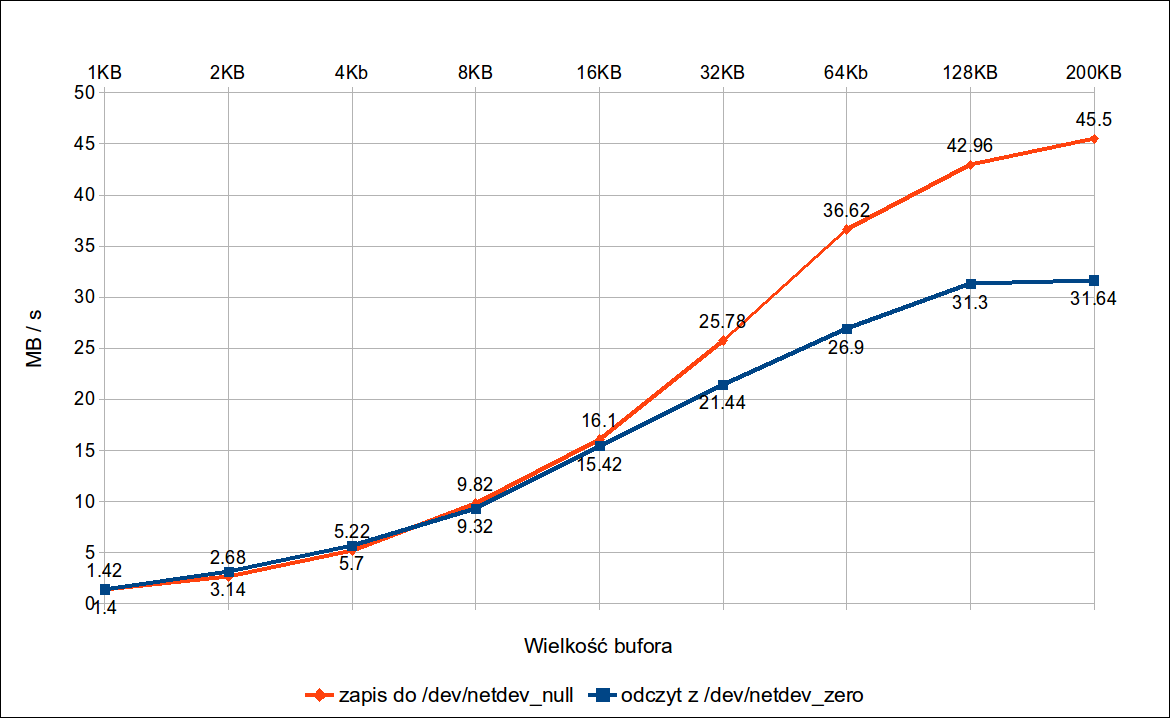
\includegraphics[width=\linewidth]{speeddevzerocomp}
\end{figure}

Od razu widoczna jest bezpośrednia zależność pomiędzy wielkością użytego bufora a prędkością jaka była osiągnięta. Im mniejszy bufor tym większy koszt wysyłania poszczególnych operacji plikowych przy pomocy protokołów Netlink oraz TCP/IP\@. Mniejszy bufor oznacza większy narzut spowodowany wielkością nagłówka i wypełnienia oraz potrzebą oczekiwania na wiadomości potwierdzające zarazem w protokole Netlink jak it TCP\@.

Zaczynając od wielkości 64 Kilobajtów wzrost wydajności transmisji zaczyna maleć a różnica pomiędzy buforami o wielkości 128 KB i 200 KB jest już nieznaczna. Oczywiście większość programów nie korzysta z buforów tak małych jak 2 czy 4 KB\@. Dla większości programów w środowisku GNU/Linux domyślna wielkość bufora odczytu to 64 KB co daje optymalną wydajność.

W przypadku zapisywania danych bufor jest zazwyczaj przystosowany do ilości jaka jest zapisywana. Jeżeli jednak ilość danych wykracza poza pojedyńcze wykonanie operacji \texttt{write()} to w tym przypadku również wielkość bufora zazwyczaj wynosi 64 KB\@. Zastanawiająca jest jednak różnica pomiędzy wydajnością operacji odczytu a operacją zapisu.

Kolejny test ma na celu porównanie wydajności odczytu z rzeczywistego urządzenia znakowego istniejącego w systemie w porównaniu do dostępu zdalnego poprzez oprogramowanie netdev. Doskonale nadającym się do tego zastosowania jest urządzenie bufora ramki \texttt{/dev/fb0}. Jest to urządzenie znakowe, które udostępnia abstrakcjny interfejs do urządzenia graficznego dostepnego w systemie\footnote{\url{http://www.tldp.org/HOWTO/Framebuffer-HOWTO/}} i jest podstawą działania konsoli dostępnej w systemach GNU/Linux tuż po załadowaniu systemu. Urządzenie to doskonale nadaje się do porównywania prędkości odczytu ponieważ udostępnia ono za każdym otwarciem tylko jedną ramkę obrazu o wielkości 50 kilobajtów i zawsze udostępnia ją z taką samą prędkością która średnio wynosi około 14.55 megabajtów na sekunde. Będzie ona dobrym punktem odniesienia dla wydajności jaką osiągnie urządzenie-atrapa.

\begin{figure}[H]
    \caption{Przepustowość odczytu z \texttt{/dev/netdev\_fb0} do \texttt{/dev/null}}
    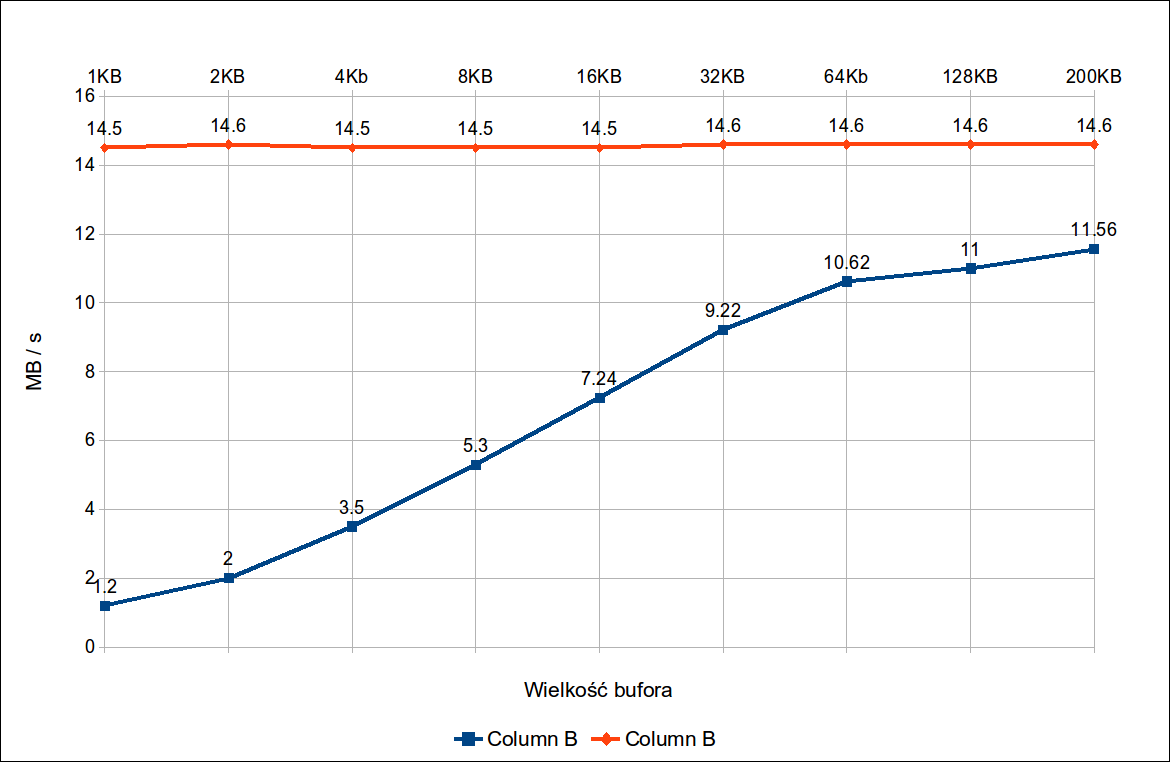
\includegraphics[width=\linewidth]{speeddevfb0}
\end{figure}

Ponownie widoczny jest ten sam trend zwiększającej się wydajności w miarę zwiększania wielkości bufora odczytu. Ponownie optymalna prędkośc osiągana jest przy buforze o wielkości 64 kilobajtów i różnice stają się coraz mnej istotne w przypadku wielkości 128 oraz 200 kilobajtów. Urządzenie-atrapa osiąga 72.7\% prędkości rzczywistego urządzenia dla 64 kilobajtów oraz odpowiednio 75.3\% i 79.2\% dla 128 i 200 kilobajtów. Jest to zadowalający wynik biorąc pod uwagę drogę jaką musi pokonać każdy odczytany bufor z danymi.

\subsection{Porównanie opóźnień}

Test

\subsection{Identyfikacja wąskich gardeł}

\subsection{Możliwe poprawki w architekturze}

\section{Podsumowanie}
\section{Dodatki}

\begin{itemize}
\itemsep1pt\parskip0pt\parsep0pt
\item
  Plik źródłowy \LaTeX z treścią pracy
\item
  Pliki graficzne diagramów oraz wykresów
\item
  Plik PDF wygenerowany na podstawie pliku LaTeX
\item
  Pełen kod źródłowy projektu w folderze \texttt{netdev}
\item
  Katalog \texttt{netdev/.git} zawierający cały opis historii rozwoju projektu
  zawarty w bazie danych systemu kontroli wersji Git
\end{itemize}

\begin{thebibliography}{99}

\bibitem{gccextensions}
    \url{http://gcc.gnu.org/onlinedocs/gcc/C-Extensions.html#C-Extensions},
    GCC Extensions.

\bibitem{asm}
    \url{http://www.ibiblio.org/gferg/ldp/GCC-Inline-Assembly-HOWTO.html#s4},
    Inline Assembly HOWTO

\bibitem{returnaddr}
    \url{http://gcc.gnu.org/onlinedocs/gcc/Return-Address.html},
    Return Address Builtin Function.

\bibitem{netlinkchange}
    \url{http://www.spinics.net/lists/netfilter-devel/msg22338.html},
    Netlink Configuration Change.

\bibitem{linuxkerneldevel}
    \textit{Linux Kernel - Przewodnik Programisty},
    Robert Love,
    2004.

\bibitem{ldd}
    \textit{Linux Device Drivers},
    Jonathan Corbet, Alessandro Rubini, Greg Kroah-Hartman,
    3rd Edition,

\bibitem{undlinuxkernel}
    \textit{Understanding Linux Kernel},
    Daniel P. Bovet, Marco Cesati,
    3rd Edtion.

\bibitem{unixnetworkprog}
    \textit{Programowanie zastosowań sieciowych w systemie UNIX},
    Richard Stevens,
    Tom 1.

\bibitem{refcount}
    \textit{Overview of Linux-Kernel Reference Counting},
    Paul E. McKenney,
    Linux Technology Center,
    IBM Beaverton,
    2007.

\bibitem{netlink}
    \textit{The Netlink protocol: Mysteries Uncovered},
    Jan Engelhardt.

\bibitem{userkernelcomm}
    \textit{Communicating between the kernel and user-space in Linux using Netlink Sockets},
    Pablo Neira Ayuso, Rafael M. Gasca, Laurent Lefevre,
    2010.

\end{thebibliography}

\listoffigures

\end{document}
